% =====================================================================
%  Proyecto Final — CS5362 Visión por Computador y Reconocimiento de Patrones
% =====================================================================
\documentclass[11pt,a4paper]{article}

% =====================================================================
%  PREÁMBULO
% =====================================================================

% --- Codificación, idioma y tipografía -------------------------------
\usepackage[utf8]{inputenc}
\usepackage[T1]{fontenc}
\usepackage{lmodern}
\usepackage{microtype}
\usepackage[spanish,es-nodecimaldot]{babel}
\addto\captionsspanish{\renewcommand{\tablename}{Tabla}\renewcommand{\listtablename}{Índice de tablas}}
\usepackage{setspace}
\setstretch{1.1}

% --- Página, encabezados y títulos -----------------------------------
\usepackage[a4paper,margin=2.5cm]{geometry}
\usepackage{fancyhdr}
\usepackage{titlesec}

\pagestyle{fancy}
\fancyhf{}
\fancyhead[L]{\small CS5362, Visión por Computador}
\fancyhead[R]{\small Proyecto Final}
\fancyfoot[C]{\thepage}
\renewcommand{\headrulewidth}{0.4pt}

\titleformat{\section}{\Large\bfseries}{\thesection.}{0.6em}{}
\titleformat{\subsection}{\large\bfseries}{\thesubsection}{0.6em}{}
\titleformat{\subsubsection}{\normalsize\bfseries\itshape}{\thesubsubsection}{0.6em}{}
\titlespacing*{\section}{0pt}{2.2ex plus 1ex}{1.2ex}
\titlespacing*{\subsection}{0pt}{1.8ex plus .5ex}{0.8ex}
\titlespacing*{\subsubsection}{0pt}{1.4ex plus .5ex}{0.6ex}

% --- Matemáticas y unidades ------------------------------------------
\usepackage{amsmath,amssymb}
\usepackage{siunitx}
\sisetup{output-decimal-marker={,}}
% Para tablas, usar columnas S[table-format=1.4] según se necesite.

% --- Figuras y tablas ------------------------------------------------
\usepackage{graphicx}
\usepackage{booktabs}
\usepackage{multirow}
\usepackage{array}
\newcolumntype{C}[1]{>{\centering\arraybackslash}p{#1}}
\newcolumntype{L}[1]{>{\raggedright\arraybackslash}p{#1}}
\usepackage{caption}
\usepackage{subcaption}
\usepackage{float}

\graphicspath{{figs/}{fotos_task_a/}{fotos_task_b/}}
\newcommand{\figwidth}{0.68\linewidth}

% --- Diagramas: TikZ y pgfplots con la paleta de la presentación ------
\usepackage[table]{xcolor}
\usepackage{tikz}
\usepackage{pgfplots}
\pgfplotsset{compat=1.18}
\usetikzlibrary{positioning,arrows.meta,calc,fit,backgrounds,shapes.geometric,babel}

% Paleta (la misma de la presentación, presentacion/estilo/tema.tex)
\definecolor{cPub}{HTML}{8A97EE}     % morado
\definecolor{cAcc}{HTML}{4F5FC8}     % morado oscuro (acento)
\definecolor{cLight}{HTML}{00BFFF}   % celeste
\definecolor{cCelD}{HTML}{0090C8}    % celeste oscuro
\definecolor{cEncBg}{HTML}{DEE2FB}   % morado claro
\definecolor{cDecBg}{HTML}{D9F4FF}   % celeste claro
\definecolor{cInk}{HTML}{2E3140}
\definecolor{cOurs}{HTML}{D92626}    % rojo (freno, la persona buscada)
\definecolor{cOursD}{HTML}{9E1B1B}
\definecolor{cUni}{HTML}{E08A2E}     % naranja
\definecolor{cSrc}{HTML}{5A5D6E}
\definecolor{cMuted}{HTML}{8A8A96}
\definecolor{cRule}{HTML}{E2E3EA}
\definecolor{cPaper}{HTML}{F5F6FA}
\definecolor{cOk}{HTML}{3C9A5F}      % verde
% estados de la carrera (Tarea A), iguales en el circuito, las fases y la máquina de estados
% Solo dos colores en los diagramas, el morado y el celeste, con sus tonos claros
\colorlet{cIda}{cAcc}
\colorlet{cFila}{cCelD}
\colorlet{cQr}{cLight}
\colorlet{cVuelta}{cPub}
% cabecera de las tablas: texto blanco sobre morado
\newcommand{\cab}[1]{\textcolor{white}{\textbf{#1}}}
\definecolor{cZebra}{HTML}{ECEEF5}   % gris leve de las filas
% tablas: cabecera morada a todo el ancho, reglas moradas pegadas a las filas
\newcommand{\tabestilo}{\small\setlength{\tabcolsep}{5pt}\renewcommand{\arraystretch}{1.25}%
  \setlength{\aboverulesep}{0pt}\setlength{\belowrulesep}{0pt}\arrayrulecolor{cAcc}}

\tikzset{
  caja/.style={draw=cInk!45, line width=0.5pt, fill=white, rounded corners=2pt, align=center,
    inner sep=3pt, font=\footnotesize, text=cInk},
  grupo/.style={draw=cInk!25, line width=0.5pt, fill=cPaper, rounded corners=3pt},
  ar/.style={-{Stealth[length=1.8mm]}, line width=0.6pt, draw=cInk!55},
  arAcc/.style={-{Stealth[length=1.8mm]}, line width=0.8pt, draw=cAcc},
  lbl/.style={font=\scriptsize, text=cSrc, align=center},
  img/.style={inner sep=0pt, draw=cRule, line width=0.4pt},
  est/.style={draw=#1, line width=0.8pt, fill=#1!10, rounded corners=6pt, font=\scriptsize\bfseries,
    text=#1!70!black, minimum height=6.5mm, inner xsep=4pt, align=center},
  estResp/.style={draw=#1, line width=0.6pt, dash pattern=on 2pt off 1.5pt, fill=white, rounded corners=6pt,
    font=\scriptsize\bfseries, text=#1!70!black, minimum height=6.5mm, inner xsep=4pt, align=center},
  % circuito visto desde arriba (figs/circuito.tex, coordenadas en m)
  pared/.style={draw=cInk!70, line width=1.3pt, line cap=round},
  senal/.style={circle, fill=white, draw=cAcc, line width=0.8pt, inner sep=0pt, minimum size=2.4mm},
  foto/.style={rectangle, fill=cMuted, draw=white, line width=0.3pt, inner sep=0pt, minimum size=1.9mm},
  buscada/.style={rectangle, fill=cAcc, draw=white, line width=0.3pt, inner sep=0pt, minimum size=2.4mm},
  puntoA/.style={diamond, fill=cInk, draw=white, line width=0.4pt, inner sep=0pt, minimum size=3mm},
  bandera/.style={rectangle, fill=white, draw=cInk, line width=0.5pt, inner sep=0pt, minimum size=3mm,
    path picture={\fill[cInk] (path picture bounding box.south west) rectangle (path picture bounding box.center)
      (path picture bounding box.center) rectangle (path picture bounding box.north east);}},
  tIda/.style={draw=cIda, line width=1pt, line join=round},
  tFila/.style={draw=cFila, line width=0.8pt, line join=round},
  tQr/.style={draw=cQr, line width=1.3pt, line join=round},
  tVuelta/.style={draw=cVuelta, line width=1pt, line join=round, dash pattern=on 2.2pt off 1.2pt},
}
% ejes sobrios para los gráficos
\pgfplotsset{
  sobrio/.style={
    axis line style={draw=cInk!45}, tick style={draw=cInk!45},
    tick label style={font=\scriptsize, text=cSrc}, label style={font=\small, text=cSrc},
    legend style={font=\scriptsize, draw=none, fill=none, text=cInk},
    grid style={draw=cRule}, major grid style={draw=cRule}, every axis plot/.append style={line width=0.9pt},
  },
}
% una fase de la línea de tiempo: \fase{desde}{hasta}{color}{texto}  (x en s, 0.9 mm por segundo)
\newcommand{\fase}[4]{%
  \fill[#3] (#1*0.9,0) rectangle (#2*0.9,6);
  \node[font=\scriptsize\bfseries, text=white] at ({(#1+#2)/2*0.9},3) {#4};}

% --- Hipervínculos (siempre al final del preámbulo) ------------------
\usepackage{hyperref}
\hypersetup{
  colorlinks=true,
  linkcolor=black,
  citecolor=black,
  urlcolor=blue,
  pdftitle={Proyecto Final - CS5362},
}

% =====================================================================
%  DOCUMENTO
% =====================================================================
\begin{document}

% ---------------------------------------------------------------------
%  Portada
% ---------------------------------------------------------------------
\begin{titlepage}
  \thispagestyle{empty}
  \centering
  \vspace*{0.5cm}
  
\includegraphics[width=5.5cm]{logo_utec.png}\par
  \vspace{1cm}

  {\large CS5362 \\[0.3em] Visión por Computador y Reconocimiento de Patrones\par}
  \vspace{1.2cm}
  \rule{\linewidth}{0.6pt}\\[0.8cm]
  {\Huge\bfseries Proyecto Final\par}
  \vspace{0.4cm}
  {\Large Attention is not all you need for robots\par}
  \vspace{0.8cm}
  \rule{\linewidth}{0.6pt}

  \vspace{1.6cm}
  {\large\bfseries Grupo 3\par}
  \vspace{0.3cm}
  {\large\bfseries Integrantes\par}
  \vspace{0.4cm}
  {\large
  Diego Randolp Quispe Apaza\\[0.3em]
  Brigitte Dayane Rojas Leon\\[0.3em]
  Alvaro Mauricio Garcia Hurtado\\[0.3em]
  Sofía del Pilar Salazar Mendoza\\[0.3em]
  Marcelino Maita Vargas\par}
  \vspace{0.8cm}
  {\large Profesor: PhD. Rensso Mora Colque\par}

  \vfill
  {\large Lima, noviembre de 2026\par}
  \vspace{1cm}
\end{titlepage}

% ---------------------------------------------------------------------
%  Índice (numeración romana)
% ---------------------------------------------------------------------
\pagenumbering{roman}
\setcounter{tocdepth}{2}
\tableofcontents
\clearpage

% ---------------------------------------------------------------------
%  Cuerpo (numeración arábiga desde 1)
% ---------------------------------------------------------------------
\pagenumbering{arabic}

% =====================================================================
\section{Introducción}
% =====================================================================

La robótica móvil busca que un robot perciba su entorno y se desplace sin ayuda humana, y para lograrlo combina sensores de distancia, como el LiDAR, con la cámara, que aporta información visual a bajo costo. En este proyecto trabajamos con un TurtleBot~4 para resolver el Desafío de Navegación Autónoma y Controlada por Gestos. El robot debe ir de un punto A a un punto B esquivando obstáculos, reconocer en B a la persona de una fotografía y volver a A anunciando su nombre.

En el laboratorio, la meta B se reconoce por una bandera a cuadros en la pared del fondo, con cuatro fotografías en los costados y un código QR en cada una, y le indicamos al robot a quién buscar para que lea el QR de esa foto y anuncie su palabra al volver. El reto tiene dos tareas. En la Tarea~A la navegación es autónoma, usa LiDAR y odometría, y corre dentro de la Raspberry Pi del robot sin depender de la red, y en la Tarea~B una persona conduce el robot con gestos de la mano, captados por la webcam de una computadora que envía las órdenes por red. En ambas tareas el robot reconoce a la persona con su cámara y conserva un freno de emergencia por LiDAR.

% =====================================================================
\section{Marco teórico}
% =====================================================================

\subsection{Robótica móvil y TurtleBot~4}

Un robot móvil repite un ciclo de percepción, decisión y acción: lee sus sensores, decide qué hacer y ejecuta un movimiento \cite{thrun2005}. El TurtleBot~4 es una plataforma educativa de base diferencial que funciona con ROS~2 e integra un LiDAR 2D, una cámara y odometría de ruedas. Se controla con la velocidad lineal $v$ y la angular $\omega$, y no puede desplazarse de lado. Su movimiento sigue el modelo cinemático
\begin{equation}
  \dot{x} = v\cos\theta, \qquad \dot{y} = v\sin\theta, \qquad \dot{\theta} = \omega,
\end{equation}
donde $(x, y)$ es la posición y $\theta$ la orientación. El enunciado permite ejecutar los algoritmos en el robot, en una computadora externa o de forma híbrida, y una computadora externa da más capacidad de cálculo y facilita la depuración, a cambio de depender de la red.

\subsection{LiDAR, odometría y SLAM}

La odometría estima la pose $(x, y, \theta)$ integrando el movimiento de las ruedas. Es simple y rápida, aunque acumula error con el tiempo, sobre todo en los giros. El LiDAR 2D mide distancias con un barrido láser a su alrededor, con buena precisión y sin depender de la iluminación. El SLAM (\textit{Simultaneous Localization and Mapping}) combina ambas fuentes para construir un mapa y estimar la pose al mismo tiempo. Cada barrido se compara con el mapa ya construido, lo que corrige la deriva de la odometría \cite{thrun2005}.

El mapa se guarda como una malla de ocupación, en la que cada celda es libre, ocupada o desconocida, y sirve de base para planificar rutas. Probamos BreezySLAM, una implementación ligera de \textit{tinySLAM} \cite{steux2010} que corre en CPU. No cierra bucles, de modo que el mapa puede desviarse en recorridos largos, y por ello en la versión final el mapa usa la odometría y la deriva se corrige al volver, como se explica en la metodología.

\subsection{Planificación de rutas y navegación reactiva}

La navegación combina un nivel global, que decide qué camino seguir, con uno local, que decide cómo seguirlo y evitar lo imprevisto. Como el circuito se conoce solo el día de la competencia, el robot debe explorar sin un mapa previo. Una opción clásica es la exploración por fronteras \cite{yamauchi1997}, donde una frontera es una celda libre pegada a una zona desconocida y se va siempre a la más cercana. Nosotros la usamos solo como respaldo.

El camino hacia un objetivo se calcula con una búsqueda en grafos sobre la malla, como Dijkstra \cite{dijkstra1959} o A* \cite{hart1968}. Inflar las paredes con el radio del robot evita rutas por donde no cabe, y el costo de pasar por una celda $c$ penaliza su cercanía a las paredes,
\begin{equation}
  C(c) = 1 + \alpha \,\max\!\left(0,\; \frac{d_{\mathrm{inf}} - d(c)}{d_{\mathrm{inf}}}\right),
\end{equation}
con $d(c)$ la distancia a la pared más cercana, $d_{\mathrm{inf}}$ el radio de influencia y $\alpha$ el peso de la penalización. Así la ruta tiende a ir por el centro de los pasillos.

Para recorrer la ruta usamos \textit{pure pursuit} \cite{coulter1992}, que persigue un punto de la ruta a una distancia $L_d$ por delante y calcula la curvatura necesaria. Si ese punto forma un ángulo $\gamma$ con la orientación del robot, entonces
\begin{equation}
  \kappa = \frac{2\sin\gamma}{L_d}, \qquad \omega = v\,\kappa .
\end{equation}
Encima de esto hay un control reactivo, que frena o gira ante un obstáculo cercano, y un freno de emergencia por LiDAR independiente del programa principal.

\subsection{Detección y reconocimiento facial}

Reconocer a una persona requiere dos etapas, encontrar la cara y decidir a quién pertenece. La detección devuelve un cuadro delimitador y cinco puntos de referencia, los ojos, la nariz y las comisuras de la boca. Usamos YuNet \cite{wu2023yunet}, un detector ligero que funciona en tiempo real en CPU. Con los cinco puntos, la cara se gira y se escala a una plantilla de $112\times112$ píxeles, lo que reduce el efecto de la rotación y la escala.

La identificación convierte la cara alineada en un vector de características (\textit{embedding}) con una red entrenada con la pérdida ArcFace \cite{deng2019arcface}, que añade un margen angular entre clases para que las caras de una misma persona queden cerca y las de personas distintas, lejos. Usamos una red ligera tipo MobileFaceNet \cite{chen2018mobilefacenets} y, de forma opcional, una ResNet-50 que rinde mejor con caras pequeñas. El vector final puede sumar el de la imagen y el de su reflejo horizontal. La similitud coseno entre el \textit{embedding} $\mathbf{q}$ de una foto del robot y el $\mathbf{g}$ de una foto de la galería es
\begin{equation}
  s(\mathbf{q},\mathbf{g}) = \frac{\mathbf{q}\cdot\mathbf{g}}{\lVert\mathbf{q}\rVert\,\lVert\mathbf{g}\rVert},
\end{equation}
y la similitud con una persona es la de su foto más parecida.

Como la persona buscada pertenece siempre a la galería, el problema es de conjunto cerrado y no hace falta un umbral de rechazo. Una sola foto puede equivocarse, así que acumulamos evidencia entre varias fotos. Para la foto $i$, la probabilidad de la persona $j$ es
\begin{equation}
  p^{(i)}_j = \frac{\exp\!\left(s^{(i)}_j/T\right)}{\sum_k \exp\!\left(s^{(i)}_k/T\right)},
\end{equation}
con una temperatura $T$ pequeña. La puntuación acumulada es $L_j = \sum_i w_i \log p^{(i)}_j$, y el peso $w_i$ crece con el tamaño de la cara, porque una cara pequeña es menos fiable. Se decide por la persona de mayor $L_j$ cuando su probabilidad supera un nivel de confianza con al menos dos fotos, o al juntar un máximo de fotos.

\subsection{Detección de manos y reconocimiento de gestos}

En la Tarea~B el robot se guía solo con gestos de la mano captados por la webcam. Un modelo de seguimiento de manos detecta en cada cuadro 21 puntos clave, la muñeca y las articulaciones de cada dedo. Usamos el detector de MediaPipe \cite{zhang2020mediapipehands}, que funciona en tiempo real y en CPU.

Con esos puntos clasificamos los gestos con geometría simple, sin entrenar un clasificador. Un dedo está estirado si su punta queda claramente más lejos de la muñeca que su articulación media, y doblado si queda más cerca. Según qué dedos estén estirados se distinguen señalar (solo el índice), una V, un puño y la mano abierta. Al señalar, la dirección del índice se compara con direcciones discretas separadas $45^\circ$, y el gesto se acepta si la diferencia es de a lo sumo $20^\circ$.

Cada gesto se traduce en una orden de movimiento, y para evitar órdenes erróneas por ruido un gesto se confirma solo si aparece en la mayoría de los últimos cuadros. La parada exige menos cuadros, porque es la acción más segura y debe actuar incluso en mitad de un giro. Una máquina de estados gobierna el movimiento, y los giros se hacen en lazo cerrado con la odometría.

\subsection{Detección y decodificación de códigos QR}

Un código QR guarda un texto en una matriz de módulos blancos y negros, con tres patrones de esquina que permiten localizarlo y orientarlo. Su lectura tiene dos pasos, detectar y rectificar el código, y luego decodificar el texto, apoyándose en la redundancia para tolerar suciedad o desenfoque. OpenCV ofrece detectores clásicos y uno basado en redes neuronales (WeChat QR). En el laboratorio cada fotografía lleva un QR junto a la cara, y aceptamos solo el que queda debajo del rostro de la persona buscada.

\subsection{Trabajos relacionados}

El SLAM con LiDAR \cite{thrun2005} y la exploración por fronteras \cite{yamauchi1997} son enfoques clásicos que funcionan en CPU y en entornos desconocidos. En reconocimiento facial se separa la detección \cite{wu2023yunet} de la identificación con \textit{embeddings} de margen angular \cite{deng2019arcface}, con modelos ligeros aptos para robots \cite{chen2018mobilefacenets}. La teleoperación visual ya se resuelve con seguimiento de manos en tiempo real \cite{zhang2020mediapipehands}. Nuestro aporte es integrar estas técnicas en un solo sistema que completa el recorrido de ida y vuelta con navegación autónoma, navegación por gestos, reconocimiento facial y lectura de QR.

% =====================================================================
\section{Metodología}
% =====================================================================

\subsection{Arquitectura general del sistema}

El sistema usa dos plataformas de cómputo conectadas por red, el robot y una computadora externa (Figura~\ref{fig:arquitectura}). El TurtleBot~4 Lite ejecuta ROS~2 en su Raspberry Pi~4 y se encarga de lo que debe responder más rápido, que es leer los sensores, mover las ruedas y frenar. Un puente que corre en el robot traduce ROS~2 a mensajes UDP, con los que se reciben los datos de los sensores y se envían las órdenes de velocidad $(v, \omega)$.

Quién decide el movimiento depende de la tarea. En la Tarea~A la navegación, el reconocimiento facial y la lectura de QR corren dentro de la Raspberry y hablan con el puente por la misma interfaz UDP. De esta forma la carrera no depende del Wi-Fi, y la computadora solo da la orden de partida y recibe el anuncio, que dice en voz alta y muestra en pantalla. En la Tarea~B, la computadora procesa la webcam para reconocer gestos, envía las órdenes de velocidad y reconoce a la persona con las fotos que pide a la cámara del robot. La computadora no usa ROS~2, de modo que su código corre en cualquier sistema operativo. El programa de la Tarea~A también puede correr en la computadora, lo que ayuda a depurar y a usar el simulador.

\begin{figure}[!t]
  \centering
  \begin{tikzpicture}[x=1mm, y=1mm]
    % --- robot
    \node[grupo, minimum width=150mm, minimum height=62mm, anchor=north west] (R) at (0,0) {};
    \node[font=\footnotesize\bfseries, text=cAcc, anchor=north west] at (3,-1.8) {Robot: TurtleBot 4 Lite (Raspberry Pi 4 y Create 3, ROS 2)};
    \node[caja, minimum width=34mm, minimum height=14mm] (se) at (22,-17) {\textbf{Sensores}\\LiDAR, odometría,\\cámara OAK-D, batería};
    \node[caja, draw=cAcc, line width=0.9pt, minimum width=44mm, minimum height=14mm] (pu) at (75,-17) {\textbf{Puente UDP}\\y \textbf{freno de emergencia}\\(LiDAR)};
    \node[caja, minimum width=24mm, minimum height=14mm] (ru) at (127,-17) {\textbf{Ruedas}\\(Create 3)};
    \draw[ar] (se) -- (pu);
    \draw[ar] (pu) -- (ru);
    \node[draw=cIda, line width=0.8pt, fill=cIda!8, rounded corners=3pt, minimum width=90mm, minimum height=25mm, anchor=north] (ta) at (50,-31) {};
    \node[font=\scriptsize\bfseries, text=cIda!70!black, anchor=north west] at ([xshift=2mm, yshift=-1mm]ta.north west) {Tarea A (autónoma, dentro de la Raspberry)};
    \node[caja, minimum width=40mm] (nav) at (28,-46.5) {Navegación\\(mapa, rutas, evasión)};
    \node[caja, draw=cAcc, line width=0.8pt, minimum width=36mm] (cqa) at (72,-46.5) {Cara y QR};
    \draw[ar, {Stealth[length=1.8mm]}-{Stealth[length=1.8mm]}] (pu.south) -- node[lbl, right] {UDP local} (pu.south |- ta.north);
    % --- computadora
    \node[grupo, minimum width=150mm, minimum height=30mm, anchor=north west] (P) at (0,-75) {};
    \node[font=\footnotesize\bfseries, text=cAcc, anchor=north west] at (3,-76.8) {Computadora (sin ROS 2)};
    \node[caja, draw=cFila, line width=0.8pt, minimum width=42mm, minimum height=13mm] (tb) at (27,-93) {\textbf{Tarea B}\\gestos de la webcam};
    \node[caja, draw=cFila, line width=0.8pt, minimum width=36mm, minimum height=13mm] (cqb) at (75,-93) {Cara y QR\\(Tarea B)};
    \node[caja, minimum width=40mm, minimum height=13mm] (an) at (123,-93) {\textbf{Anuncio} y salida\\voz, pantalla, START};
    % --- red
    \draw[ar, {Stealth[length=1.8mm]}-{Stealth[length=1.8mm]}, draw=cAcc, line width=0.9pt] (108,-62) -- node[lbl, right, xshift=1mm] {UDP por Wi-Fi:\\datos $\downarrow$\\órdenes $\uparrow$} (108,-75);
  \end{tikzpicture}
  \caption{Arquitectura general. El robot se encarga de los sensores, las ruedas y el freno de emergencia, y en la Tarea~A también de la navegación y el reconocimiento. La computadora procesa los gestos de la Tarea~B y se comunica con el robot por UDP. Morado: Tarea~A; celeste: Tarea~B.}
  \label{fig:arquitectura}
\end{figure}

El diseño separa la seguridad de la decisión. Si el programa que decide falla o se pierde la conexión, el puente mantiene un freno de emergencia por LiDAR que detiene al robot a \SI{0,28}{\meter} de un obstáculo al frente. La velocidad enviada se limita al máximo del robot, \SI{0,31}{\meter\per\second}, o \SI{0,46}{\meter\per\second} en la vuelta turbo de la Tarea~A. El código se organiza en módulos independientes (comunicación, navegación de cada tarea y reconocimiento), que se prueban por separado, y las dos tareas comparten los de comunicación y reconocimiento.

\subsection{Integración de sensores}

El robot entrega tres fuentes de información, que resume la Tabla~\ref{tab:sensores}, y además informa su batería. El LiDAR da las distancias a paredes y obstáculos, y sirve para el mapa y el freno. La odometría da la pose y sirve para ubicar el robot, trazar su recorrido y hacer los giros en lazo cerrado. La cámara da las fotos de señales, bandera, personas y QR, y la webcam de la computadora es un sensor aparte, usado solo en la Tarea~B. En la Tarea~A el mapa se construye con la odometría y el LiDAR corrige su deriva al volver a A. En la Tarea~B no hay mapa, porque el robot solo gira un ángulo conocido y avanza recto.

\begin{table}[!htbp]
  \centering
  \caption{Sensores usados y su función en cada tarea.}
  \label{tab:sensores}
  \tabestilo
  \rowcolors{2}{cZebra}{white}
  \begin{tabular}{L{3.0cm}L{3.7cm}L{3.7cm}L{3.7cm}}
    \toprule
    \rowcolor{cAcc}\cab{Sensor} & \cab{Dato} & \cab{Tarea A} & \cab{Tarea B} \\
    LiDAR 2D & Distancias en $360^\circ$ (720 puntos, unos \SI{7}{\hertz}) & Mapa, planificación, evasión y freno & Freno de emergencia y distancia libre al frente \\
    Odometría & Pose $(x, y, \theta)$ & Localización, seguimiento de ruta y relocalización & Giros en lazo cerrado y rumbo \\
    Cámara del robot & Fotos a color, vista previa y HD & Señales; bandera, caras y QR en la meta & Cara y QR durante la conducción \\
    Webcam & Imagen de la mano & No se usa & Reconocimiento de gestos \\
    \bottomrule
  \end{tabular}
\end{table}

Cada flujo llega con un ritmo y un retraso distintos, así que un hilo independiente recibe cada uno y guarda solo el último dato, que el programa principal lee cuando lo necesita. De este modo no se acumulan datos viejos. La Raspberry procesa unas dos fotos de la vista previa por segundo en la Tarea~A, y una foto HD tarda unos \SI{4}{\second} en llegar. La computadora de la Tarea~B pide unas cuatro fotos por segundo, y el reconocimiento corre en su propio hilo para no frenar el control. El freno por LiDAR solo vigila el frente, por lo que un obstáculo a los costados o detrás no lo activa. En la Tarea~A fusionamos además la cámara y el LiDAR, de modo que el rumbo de una cara, una flecha o la bandera sale de la imagen, su distancia sale del LiDAR en ese rumbo y cada una queda ubicada en el mapa.

\subsection{Reconocimiento facial y lectura de QR}

El módulo es común a ambas tareas y corre en CPU solo con OpenCV (Figura~\ref{fig:pipeline_cara}). Usa dos formatos de la cámara OAK-D Lite, montada a unos \SI{13}{\centi\meter} del suelo. La vista previa de $250\times250$ píxeles ($42^\circ$ de campo) es liviana y rápida, y la foto HD de $1280\times720$ píxeles ($69^\circ$) da caras unas tres veces más grandes. La HD se pide para leer el QR y para confirmar de cerca una cara que salió chica en la vista previa.

\begin{figure}[!htbp]
  \centering
  \begin{tikzpicture}[x=1mm, y=1mm, l/.style={font=\scriptsize, text=cInk, align=center}]
    \useasboundingbox (0,12) rectangle (150,-48);
    \node[img] (r) at (12.5,0) {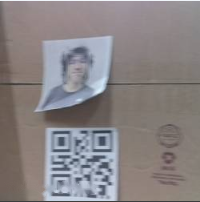
\includegraphics[height=22mm]{robot_limpia.png}};
    \node[img] (y) at (45,0) {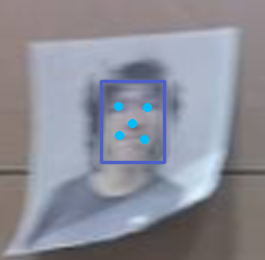
\includegraphics[height=22mm]{cara_yunet.png}};
    \node[img] (a) at (76,0) {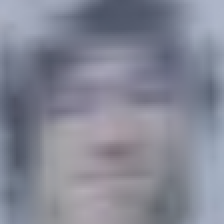
\includegraphics[height=15mm]{cara_alineada.png}};
    \node[img] (e) at (106,0) {
\includegraphics[width=20mm, height=5mm]{embedding.png}};
    \node[font=\bfseries, text=cAcc, align=center] (n) at (137,0) {Thiago\\[-0.5mm]Frias};
    \draw[ar] (r) -- (y);
    \draw[ar] (y) -- (a);
    \draw[ar] (a) -- (e);
    \draw[ar] (e) -- (n);
    \node[l, below=1.5mm of r] {cámara del robot};
    \node[l, below=1.5mm of y] {\textbf{YuNet}\\caja y 5 puntos};
    \node[l, below=6mm of a] {alinear\\$112\times112$};
    \node[l, below=1.5mm of e] {\textbf{ArcFace}\\512 números};
    \node[l, below=1.5mm of n] {la más parecida\\de 20 personas};
    % segunda fila: de la imagen al anuncio
    \node[caja, draw=cAcc, minimum width=31mm, minimum height=10mm] (v) at (20.5,-42) {\textbf{Votación} entre fotos\\pesada por el tamaño};
    \node[caja, draw=cAcc, minimum width=31mm, minimum height=10mm] (c) at (59.5,-42) {\textbf{Confirmar de cerca}\\foto HD si la cara $<40$\,px};
    \node[caja, draw=cCelD, line width=0.8pt, minimum width=31mm, minimum height=10mm] (q) at (98.5,-42) {\textbf{QR} debajo de\\la cara buscada};
    \node[caja, draw=cCelD, line width=0.8pt, minimum width=23mm, minimum height=10mm] (p) at (133.5,-42) {\textbf{Anuncio}\\nombre y palabra};
    \draw[ar] (v) -- (c);
    \draw[ar] (c) -- (q);
    \draw[ar] (q) -- (p);
  \end{tikzpicture}
  \caption{Módulo de reconocimiento facial y de QR. Arriba se ve el reconocimiento de una foto, sobre una captura real de la cámara del robot, y abajo cómo se decide con varias fotos y se obtiene la palabra.}
  \label{fig:pipeline_cara}
\end{figure}

\subsubsection{Detección del rostro}

Usamos YuNet (\texttt{cv2.FaceDetectorYN}) con umbral de confianza $0{,}6$. YuNet pierde las caras de menos de unos 20 píxeles, así que ampliamos la vista previa $\times 2$ (lado menor de 500 píxeles) antes de detectar. Esto permite ver caras de unos 12 píxeles y cuesta cuatro veces más cálculo. Si bien ampliar solo a 320 píxeles era 2,6 veces más barato, en simulación las carreras exitosas bajaron de 19 a 13 de 25. Con los cinco puntos alineamos la cara a $112\times112$ píxeles. Las fotos tomadas girando a más de \SI{1}{\radian\per\second} salen movidas y no se reconocen.

\subsubsection{Identificación de la persona}
\label{sec:ident}

ArcFace convierte cada cara en un vector de 512 dimensiones. Usamos MobileFaceNet (\SI{13}{\mega\byte}) por defecto y, de forma opcional, ResNet-50 (\SI{174}{\mega\byte}), ambas entrenadas en WebFace600K. La galería tiene 20 personas y 110 fotos. La votación usa $T = 0{,}04$ y un peso por ancho de cara $a$ en píxeles,
\begin{equation}
  w = \min\!\left(1,\; \max\!\left(0{,}15,\; \frac{a - 14}{42}\right)\right).
\end{equation}
En general se decide cuando el líder supera $p = 0{,}97$ con al menos dos fotos, o al juntar ocho.

En la Tarea~A no sumamos el vector del reflejo, lo que reduce a la mitad el costo de ArcFace en la Raspberry y casi no cambia el acierto, que a 24 píxeles es de \SI{95,8}{\percent} por foto frente a \SI{96,2}{\percent} con el reflejo (Sección~\ref{sec:res_cara}). En la meta hay cuatro fotos y cada una tiene su propia votación. Solo votan las vistas de frente, ponderadas por $\cos^2$ del ángulo con la normal de la pared y descartadas por encima de $55^\circ$. Además, solo cuentan las caras a menos de \SI{2,2}{\meter} de la bandera y de \SI{0,5}{\meter} del piso, para ignorar a las personas del laboratorio.

Una foto se declara la buscada de inmediato si, en dos vistas, su probabilidad es $p \ge 0{,}90$ y la cara mide al menos 24 píxeles. Si no, al terminar la vuelta de la meta hacemos un ranking sin umbral, vamos a la foto más parecida a la persona buscada y la confirmamos de cerca. De cerca, la buscada debe ganar con $p \ge 0{,}45$ y una cara de al menos 24 píxeles. Si en la vista previa la cara mide menos de 40 píxeles, se piden fotos HD y se decide con ellas, hasta \SI{11}{\second} por foto. Si de cerca gana otra persona con $p \ge 0{,}6$, la foto se descarta y se pasa a la siguiente. Si no se sabe quién es, la foto queda como dudosa y se revisan primero las demás. Cuando quedan descartadas las otras tres, la que sobra es la buscada. En la Tarea~B conservamos el reflejo, reiniciamos la votación tras \SI{4}{\second} sin ver una cara y descartamos a cualquier persona distinta de la buscada.

\subsubsection{Lectura del QR}

Combinamos dos lectores de OpenCV, el clásico (\texttt{QRCodeDetector}), que se aplica a zonas ampliadas debajo y a los costados de cada cara, y el de WeChat, basado en redes neuronales, que se aplica a la imagen entera y lee códigos de unos 2 píxeles por módulo. Como las fotos de la meta están en fila, hay que saber de qué cara es cada QR. Para esto medimos la distancia horizontal al centro de la cara en anchos de cara $a$. El QR propio queda a menos de $1{,}6\,a$ y el de la foto vecina, a más de $2{,}5\,a$, y asignamos un QR a una cara si está debajo de su centro y a no más de $2{,}0\,a$ hacia el costado.

Una palabra equivocada se penaliza. Por eso, en la Tarea~A solo aceptamos un texto asignado a la cara que la misma foto reconoce como la buscada, leído dos veces (una si la cara mide al menos 35 píxeles) y nunca visto junto a otra persona. El robot se pone de frente a la foto a unos \SI{0,65}{\meter}, retrocediendo antes un poco porque de cerca el QR, que va debajo de la foto, queda fuera del cuadro, y pide la foto HD enseguida. Si en \SI{30}{\second} no logra leerlo, vuelve a A y anuncia solo el nombre. En la Tarea~B el QR se busca sin límite de tiempo tras reconocer a la persona.

\subsection{Navegación autónoma (Tarea~A)}

La solución prioriza el tiempo, ya que el puntaje depende de él, y por eso el robot no hace un barrido inicial ni explora todo el mapa. Sale por el espacio más abierto, sigue las señales de giro hasta ver la bandera, mira las cuatro fotos desde el centro del último tramo, confirma de cerca la que parece la buscada, lee su QR y vuelve por el camino más corto. La Figura~\ref{fig:estados} muestra la máquina de estados, con los estados IDA, META, ACERCAR, RECONOCER, LEER\_QR, VOLVER y HECHO, y dos respaldos, FILA y EXPLORAR. El mismo programa corre dentro de la Raspberry en la competencia y también en la computadora.

\begin{figure}[!htbp]
  \centering
  \begin{tikzpicture}[x=1mm, y=1mm]
    \node[est=cIda, minimum width=20mm] (ida) at (0,0) {IDA};
    \node[est=cFila, minimum width=20mm] (meta) at (40,0) {META};
    \node[est=cFila, minimum width=22mm] (ace) at (80,0) {ACERCAR};
    \node[est=cFila, minimum width=24mm] (rec) at (120,0) {RECONOCER};
    \node[est=cFila, minimum width=24mm] (qr) at (120,-28) {LEER\_QR};
    \node[est=cIda, minimum width=22mm] (vol) at (60,-28) {VOLVER};
    \node[est=cIda, minimum width=20mm] (fin) at (0,-28) {HECHO};
    \node[estResp=cIda, minimum width=22mm] (exp) at (0,19) {EXPLORAR};
    \node[estResp=cFila, minimum width=20mm] (fila) at (60,19) {FILA};
    \draw[ar] (ida) -- node[lbl, above] {bandera} (meta);
    \draw[ar] (meta) -- node[lbl, above] {ranking} (ace);
    \draw[ar] (ace) -- node[lbl, above] {de frente} (rec);
    \draw[ar] (rec) -- node[lbl, right] {es la buscada} (qr);
    \draw[ar] (qr) -- node[lbl, above] {QR o 30 s} (vol);
    \draw[ar] (vol) -- node[lbl, above] {en A} (fin);
    \draw[ar, dash pattern=on 2pt off 1.5pt] (ida) -- node[lbl, right] {25 s sin\\sitios nuevos} (exp);
    \draw[ar, dash pattern=on 2pt off 1.5pt] (meta.north) |- node[lbl, left, pos=0.25] {no se\\resuelve} (fila.west);
    \draw[ar, dash pattern=on 2pt off 1.5pt] (fila.east) -| (ace.north);
    \draw[ar] (rec.south west) to[bend left=28] node[lbl, below, pos=0.5] {descartada o dudosa:\\siguiente foto} (ace.south east);
  \end{tikzpicture}
  \caption{Máquina de estados de la Tarea~A. Morado: navegación por el camino; celeste: trabajo en la meta. Los estados con línea punteada son los respaldos.}
  \label{fig:estados}
\end{figure}

\subsubsection{Mapeo y localización (SLAM)}

El mapa es una malla de ocupación de $500\times500$ celdas de \SI{4}{\centi\meter}, con valores \textit{log-odds}. Cada barrido suma 20 a las celdas donde termina un rayo y resta 6 a las que atraviesa, de modo que una pared aparece enseguida y no se borra por una lectura perdida. La pose viene de la odometría de la Create~3, porque BreezySLAM corrige bien solo con movimientos lentos y en una sala de $4\times4$~m la odometría basta durante la ida.

La deriva se corrige al volver. El robot guarda el barrido del LiDAR en A y, al estar de vuelta a menos de \SI{2}{\meter} de A, lo alinea con el actual mediante ICP~2D. Aceptamos la corrección si el error medio es menor a \SI{6}{\centi\meter}, se emparejan más del 45\,\% de los puntos y el ajuste es menor a \SI{0,8}{\meter} y $30^\circ$.

\subsubsection{Ida con carriles y señales}

En la IDA el robot elige en cada paso un \textit{carril} entre rumbos separados $5^\circ$, el que tiene espacio libre según el LiDAR, sigue la dirección de avance o de una señal y no lleva a zonas ya recorridas. Las señales son discos con una flecha negra, azules para la ida y rojos para la vuelta, y hay también discos lisos y señales de prohibido.

Detectamos las flechas sin entrenamiento (Figura~\ref{fig:sim_flecha}), y para ello pasamos la imagen al canal $\min(B,G,R)$, donde una flecha negra queda oscura aunque esté sobre un disco de color, buscamos manchas rodeadas de papel claro y las comparamos con plantillas sintéticas de flechas y de formas que no lo son, como aros, el símbolo de prohibido y cruces. Una señal se confirma con dos fotos y el robot gira al llegar junto a ella. Los discos rojos, los lisos y el de prohibido se ignoran, porque la vuelta usa el camino recorrido. Con 540 fotos reales de la cámara del TurtleBot de otros semestres, usadas solo para medir, el detector acierta el \SI{89}{\percent} de las flechas izquierdas y el \SI{86}{\percent} de las derechas por foto, rechaza bien el \SI{97}{\percent} de las fotos sin flecha y nunca se equivoca de sentido.

\begin{figure}[!htbp]
  \centering
  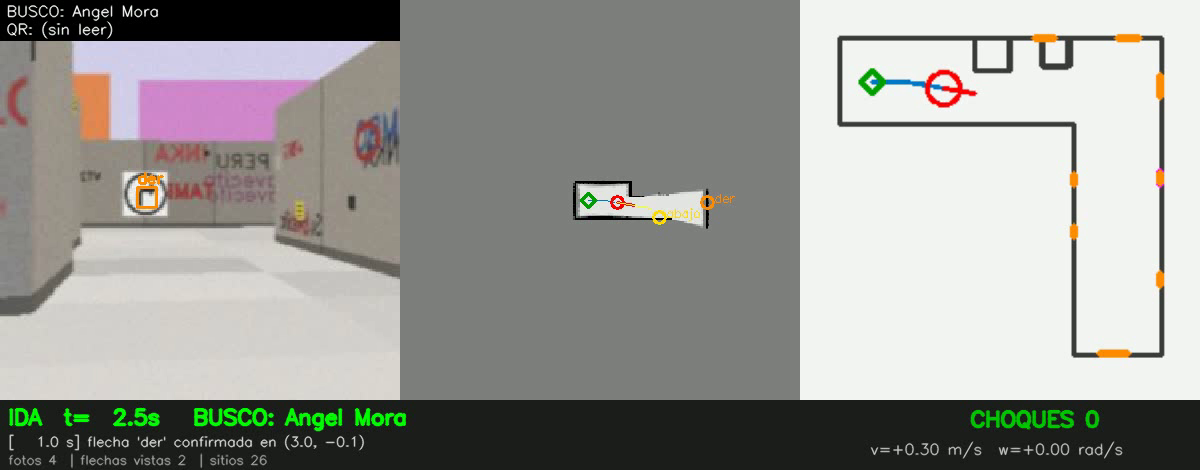
\includegraphics[width=0.92\linewidth]{sim_flecha.png}
  \caption{Simulación de la Tarea~A. A la izquierda se ve la cámara del robot con una señal de giro detectada, en el centro el mapa construido con el LiDAR y a la derecha el circuito con el recorrido.}
  \label{fig:sim_flecha}
\end{figure}

\subsubsection{La meta con bandera y cuatro fotos}

En la meta, una bandera a cuadros va pegada en la pared del fondo del último tramo y las cuatro fotos van en los costados, dos de cada lado. Detectamos la bandera sin entrenamiento. Buscamos una mancha de muchos cuadros negros parejos, pegados en diagonal sobre papel claro, donde la tinta y el papel alternan al menos cuatro veces por fila y tres por columna. Un QR o un texto no cumplen esto, porque sus cuadros tienen tamaños muy distintos. Además, la hoja va sobre una caja de cartón, lo que usamos como indicio. En unos 1000 cuadros de tres videos del laboratorio solo marcó la bandera de verdad. La confirmamos con dos vistas si la hoja está sobre cartón, y con cuatro si no. Una bandera a menos de \SI{1}{\meter} de A es la de la salida, y si desde el centro del tubo no se ve ninguna foto, esa bandera no es la meta.

Con la bandera confirmada el robot pasa a META (Figura~\ref{fig:meta}), va al centro del tubo, a \SI{0,65}{\meter} del fondo, y da una vuelta lenta (\SI{0,4}{\radian\per\second}) con seis paradas, a $\pm45^\circ$, $\pm90^\circ$ y $\pm135^\circ$ de la bandera, sin detenerse a mirar hacia atrás. En cada parada queda quieto al menos \SI{1,2}{\second} y hasta recibir tres fotos (como máximo \SI{2,5}{\second}), porque girando a más de \SI{1}{\radian\per\second} las fotos salen movidas. Al terminar la vuelta se hace el ranking de las fotos vistas y se confirman de cerca, como se explicó en la Sección~\ref{sec:ident}. Si no se vieron las cuatro fotos, el robot hace una segunda vuelta a \SI{1,4}{\meter} del fondo, porque en un tubo largo las fotos quedan más atrás. Si todavía no se resuelve, pasa al respaldo FILA y, como último recurso, lee el QR de la foto más parecida. Si en \SI{100}{\second} no ha visto la bandera, cualquier cara cuenta.

\begin{figure}[!htbp]
  \centering
  \begin{subfigure}[b]{0.31\linewidth}
    \centering
    \begin{tikzpicture}[x=1.15mm, y=1.15mm]
      \fill[cPaper] (0,0) rectangle (22,56);
      \draw[pared] (0,56) -- (0,0) -- (22,0) -- (22,56);
      \node[bandera] at (11,1.6) {};
      \node[foto, minimum size=2.4mm] at (0.9,34) {};
      \node[foto, minimum size=2.4mm] at (0.9,20) {};
      \node[foto, minimum size=2.4mm] at (21.1,44) {};
      \node[buscada, minimum size=2.8mm] at (21.1,26) {};
      \draw[cFila, line width=0.4pt, dash pattern=on 1pt off 1pt] (11,16) circle (7);
      \foreach \a/\n in {-45/1, 0/2, 45/3, 135/4, 180/5, -135/6}{
        \draw[cFila, line width=0.6pt, -{Stealth[length=1mm]}] (11,16) -- ++(\a:7);
        \node[circle, draw=cFila, fill=white, line width=0.5pt, inner sep=0pt, minimum size=3mm,
              font=\fontsize{5.5}{5.5}\selectfont\bfseries, text=cFila] at ($(11,16)+(\a:11)$) {\n};}
      \draw[cInk, fill=white, line width=0.6pt] (11,16) circle (2.4);
      \draw[cInk, line width=0.8pt, -{Stealth[length=1.1mm]}] (11,16) -- (11,13.6);
      \draw[cIda, line width=1pt, -{Stealth[length=1.4mm]}] (11,63) -- (11,57);
      \draw[<->, cSrc, line width=0.4pt] (-3.5,0) -- node[lbl, left] {\SI{0,65}{\meter}} (-3.5,16);
      \node[lbl, below=0.5mm] at (11,-0.5) {bandera};
    \end{tikzpicture}
    \caption{Esquema visto desde arriba.}
  \end{subfigure}
  \hfill
  \begin{subfigure}[b]{0.66\linewidth}
    \centering
    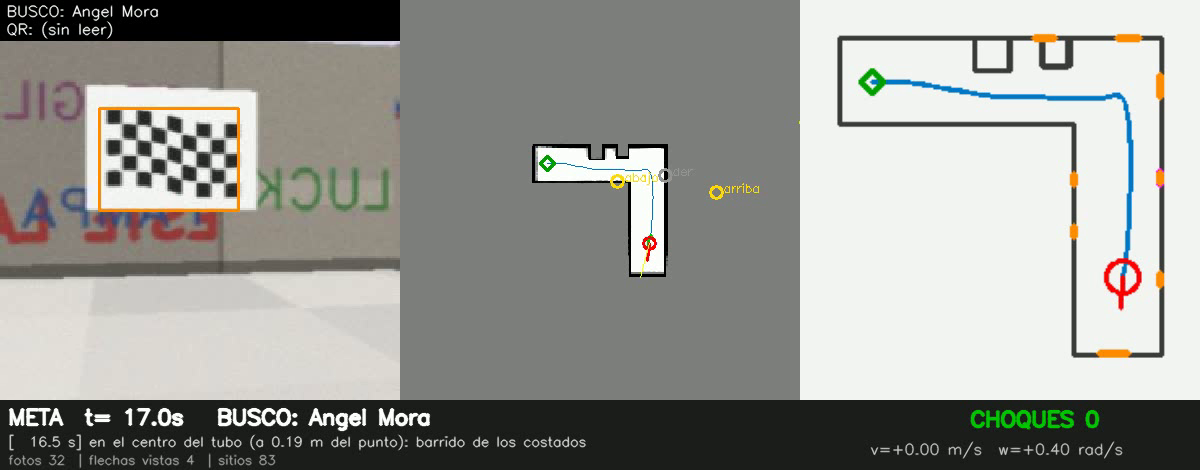
\includegraphics[width=\linewidth]{sim_bandera.png}
    \caption{Simulación con la bandera detectada (recuadro naranja).}
  \end{subfigure}
  \caption{Estado META. El robot va al centro del tubo frente a la bandera y da una vuelta lenta con seis paradas numeradas, para que las cuatro fotos de los costados pasen por el campo de la cámara. La foto buscada se marca en morado.}
  \label{fig:meta}
\end{figure}

\subsubsection{Respaldos de fila de fotos y exploración}

En FILA, el robot arma puntos de vista a unos \SI{0,5}{\meter} de la pared y mira las fotos una por una hasta encontrar a la buscada. Si pasan \SI{25}{\second} sin descubrir sitios nuevos, activa el plan~B, que es la exploración por fronteras con Dijkstra y \textit{pure pursuit}.

\subsubsection{Vuelta, seguimiento de ruta y evasión de obstáculos}

Para VOLVER usamos la ruta más corta a A según el mapa, calculada con Dijkstra. Si el robot no avanza en \SI{8}{\second}, desanda la ida punto por punto. El rumbo elegido se convierte en $(v,\omega)$ con una ventana dinámica, en la que simulamos 114 arcos de \SI{1,2}{\second}, 20 veces por segundo, y descartamos los que pasan a menos de \SI{20}{\centi\meter} de un obstáculo o entran en la zona de freno del puente. Entre los arcos seguros elegimos el que más avanza hacia el rumbo. De esta forma el robot va a \SI{0,30}{\meter\per\second} en las rectas y frena solo cerca de paredes o en los giros. Si en \SI{3}{\second} no avanza \SI{6}{\centi\meter}, se desvía hacia el carril más abierto, y si queda pegado de frente, retrocede unos \SI{14}{\centi\meter}.

En la vuelta, por un camino ya conocido, usamos el modo turbo. La velocidad sube a \SI{0,45}{\meter\per\second}, para lo cual quitamos el límite de fábrica de la Create~3 (\texttt{safety\_override} en \texttt{full}) y el puente admite hasta \SI{0,46}{\meter\per\second}. El punto de mira se adelanta a $0{,}6 + 1{,}6\,(v - 0{,}2)$ metros, así que el robot empieza a doblar antes y en curva, y la ventana dinámica sigue revisando cada arco contra el LiDAR. En simulación la vuelta baja de \SI{17,1}{\second} a \SI{12,3}{\second} de mediana (\SI{-28}{\percent}) sin choques.

\subsubsection{Freno de emergencia y seguridad}

La seguridad tiene capas independientes. El puente frena con un obstáculo a menos de \SI{0,28}{\meter} en un pasillo de $\pm\SI{0,20}{\meter}$ al frente y no suelta hasta tener \SI{0,38}{\meter} libres. El navegador lleva una copia de ese freno para no pedir arcos que el puente anularía. Además, el programa arranca en pausa y la barra espaciadora detiene al robot de inmediato.

\subsection{Navegación por gestos (Tarea~B)}

\subsubsection{Captura y reconocimiento de gestos}

La persona se ubica frente a la webcam de la computadora, configurada a $640\times480$ píxeles en MJPG. No usamos una resolución mayor, porque el detector de manos no mejora con ella y el procesamiento sería más lento. Un hilo lee la cámara y entrega siempre el cuadro más reciente, de modo que no se acumulan cuadros viejos. La imagen se voltea como un espejo (vista \textit{selfie}), y en cada cuadro MediaPipe, con una sola mano, entrega los 21 puntos clave. Este modelo no requiere entrenamiento propio.

\begin{figure}[!htbp]
  \centering
  \begin{tikzpicture}[x=1mm, y=1mm]
    \node[caja, minimum width=27mm, minimum height=12mm] (w) at (0,0) {\textbf{Webcam}\\$640\times480$, MJPG};
    \node[caja, minimum width=31mm, minimum height=12mm, right=6mm of w] (m) {\textbf{MediaPipe}\\21 puntos de la mano};
    \node[caja, minimum width=31mm, minimum height=12mm, right=6mm of m] (g) {\textbf{Reglas}\\dedos estirados\\y dirección};
    \node[caja, draw=cFila, line width=0.8pt, minimum width=30mm, minimum height=12mm, right=6mm of g] (e) {\textbf{Estabilizador}\\5 de 8 cuadros\\(STOP: 2 de 8)};
    \draw[ar] (w) -- (m);
    \draw[ar] (m) -- (g);
    \draw[ar] (g) -- (e);
    \node[grupo, minimum width=137mm, minimum height=34mm, anchor=north west] (ctl) at (-13.5,-20) {};
    \node[font=\scriptsize\bfseries, text=cAcc, anchor=north west] at (-11.5,-21.2) {Control: máquina de estados con la odometría};
    \node[est=cSrc, minimum width=22mm] (par) at (10,-42) {PARADO};
    \node[est=cFila, minimum width=22mm] (gir) at (62,-42) {GIRANDO};
    \node[est=cIda, minimum width=26mm] (ava) at (114,-42) {AVANZANDO};
    \draw[ar] (e.south) -- node[lbl, right] {gesto confirmado} (e.south |- ctl.north);
    \draw[ar] (par.east) to[bend left=22] node[lbl, above] {señalar} (gir.west);
    \draw[ar] (gir.west) to[bend left=22] node[lbl, below] {giro hecho} (par.east);
    \draw[ar] (gir.east) to[bend left=22] node[lbl, above] {V o puño} (ava.west);
    \draw[ar] (ava.west) to[bend left=22] node[lbl, below] {señalar} (gir.east);
    \draw[ar, draw=cAcc] (ava.north) -- ++(0,5) -- node[lbl, above, text=cAcc] {mano abierta (STOP), desde cualquier estado} ($(par.north)+(0,5)$) -- (par.north);
  \end{tikzpicture}
  \caption{Tarea~B, del cuadro de la webcam a la orden de movimiento. El robot arranca parado y la parada tiene prioridad sobre cualquier otro gesto.}
  \label{fig:pipeline_gestos}
\end{figure}

Con esos puntos, un clasificador geométrico decide el gesto sin redes adicionales. Un dedo está estirado si la distancia de su punta a la muñeca supera en un 15\,\% la de su articulación media, y doblado si es menor. El pulgar no interviene. Las reglas reconocen cuatro gestos (Tabla~\ref{tab:gestos}). Al señalar, el ángulo del índice se compara con siete direcciones separadas $45^\circ$, todas menos la vertical hacia arriba, y se acepta si la diferencia es de a lo sumo $20^\circ$. Entre dos direcciones queda un hueco que no cuenta como gesto, así que el reconocimiento no salta de una a otra. El índice hacia arriba no es un gesto, porque esa dirección se reserva para la V y la mano abierta. La V se acepta solo con la mano hacia arriba ($\pm40^\circ$), y la mano abierta se reconoce en cualquier orientación, para poder cortar un giro sin girar la mano.

\begin{table}[!htbp]
  \centering
  \caption{Gestos reconocidos y acción asociada del robot.}
  \label{tab:gestos}
  \tabestilo
  \rowcolors{2}{cZebra}{white}
  \begin{tabular}{L{3.2cm}L{5.6cm}L{5.6cm}}
    \toprule
    \rowcolor{cAcc}\cab{Gesto} & \cab{Condición geométrica} & \cab{Acción del robot} \\
    Señalar con el índice & Solo el índice estirado, en una de las siete direcciones & Gira $45^\circ$, $90^\circ$, $135^\circ$ o $180^\circ$ hacia ese lado y se detiene \\
    V (índice y corazón) & Ambos estirados hacia arriba ($\pm 40^\circ$) & Avanza lento (\SI{0,15}{\meter\per\second}) \\
    Puño & Los cuatro dedos doblados & Avanza rápido (\SI{0,31}{\meter\per\second}, el máximo del robot) \\
    Mano abierta & Los cuatro dedos estirados, en cualquier dirección & Se detiene de inmediato, incluso en pleno giro \\
    \bottomrule
  \end{tabular}
\end{table}

Para filtrar el ruido, un estabilizador confirma un gesto cuando aparece en 5 de los últimos 8 cuadros. La parada exige solo 2 de 8, porque es el gesto de seguridad y debe responder más rápido. Un gesto confirmado se mantiene hasta que casi desaparece de la ventana. Cuando no hay mano, el sistema no genera ningún evento y el robot continúa con la última acción. La Figura~\ref{fig:gestos} muestra la ventana del programa con cada gesto.

\begin{figure}[!htbp]
  \centering
  \begin{subfigure}[t]{0.32\linewidth}
    \centering
    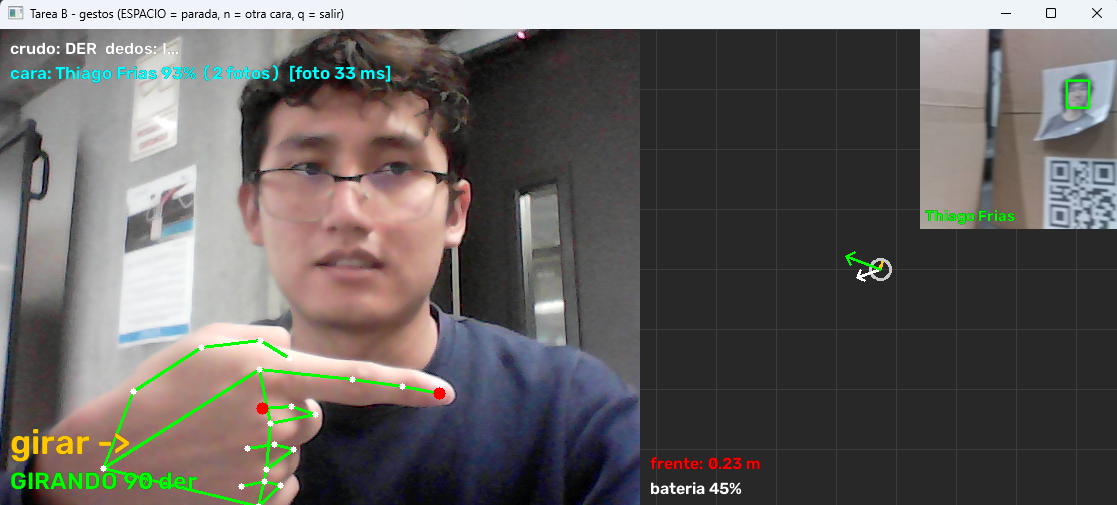
\includegraphics[width=\linewidth]{girar_derecha.png}
    \caption{Señalar a la derecha.}
  \end{subfigure}
  \hfill
  \begin{subfigure}[t]{0.32\linewidth}
    \centering
    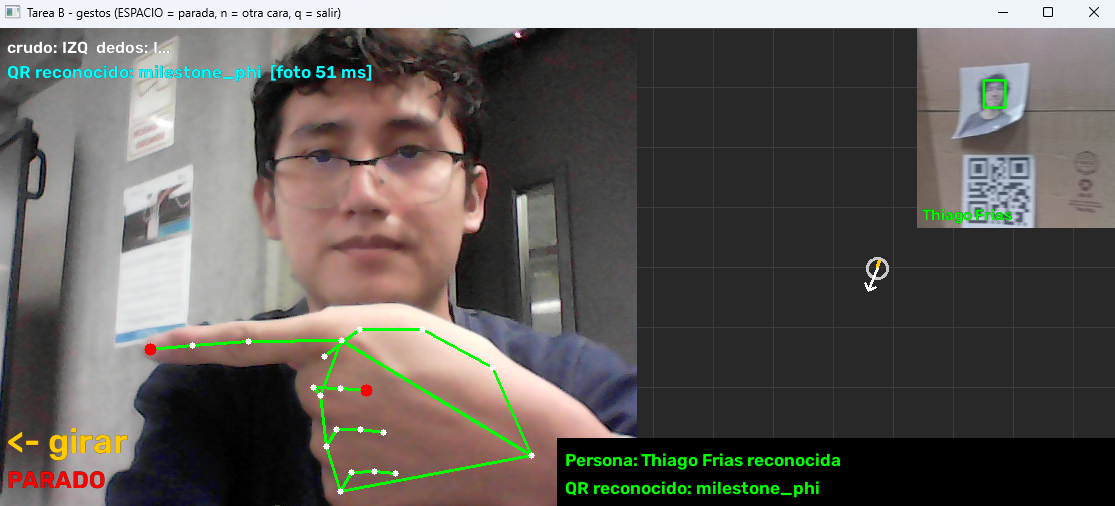
\includegraphics[width=\linewidth]{girar_izquierda.png}
    \caption{Señalar a la izquierda.}
  \end{subfigure}
  \hfill
  \begin{subfigure}[t]{0.32\linewidth}
    \centering
    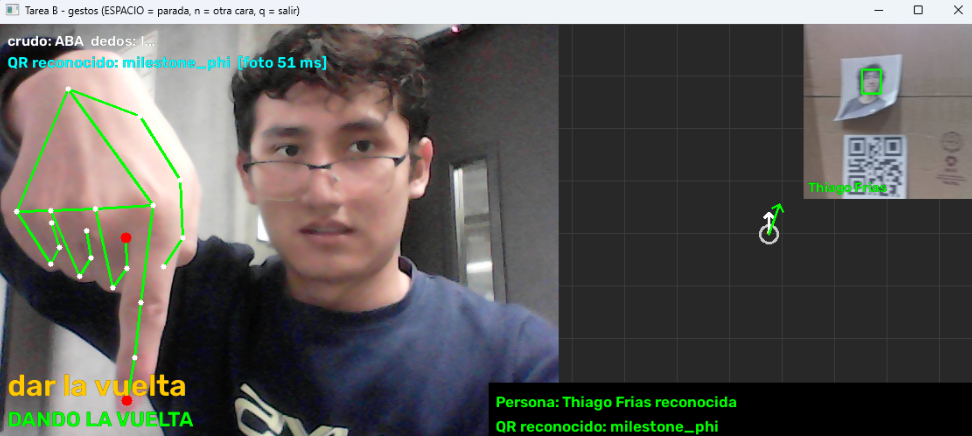
\includegraphics[width=\linewidth]{dar_la_vuelta.png}
    \caption{Señalar abajo.}
  \end{subfigure}

  \vspace{0.4em}
  \begin{subfigure}[t]{0.32\linewidth}
    \centering
    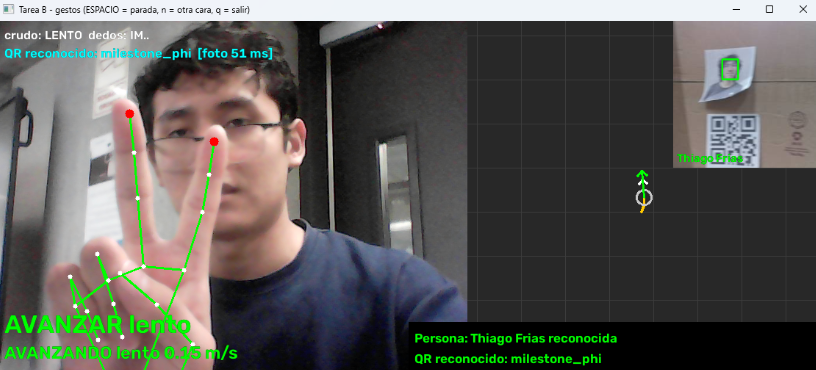
\includegraphics[width=\linewidth]{avanzar_lento.png}
    \caption{V, avanza lento.}
  \end{subfigure}
  \hfill
  \begin{subfigure}[t]{0.32\linewidth}
    \centering
    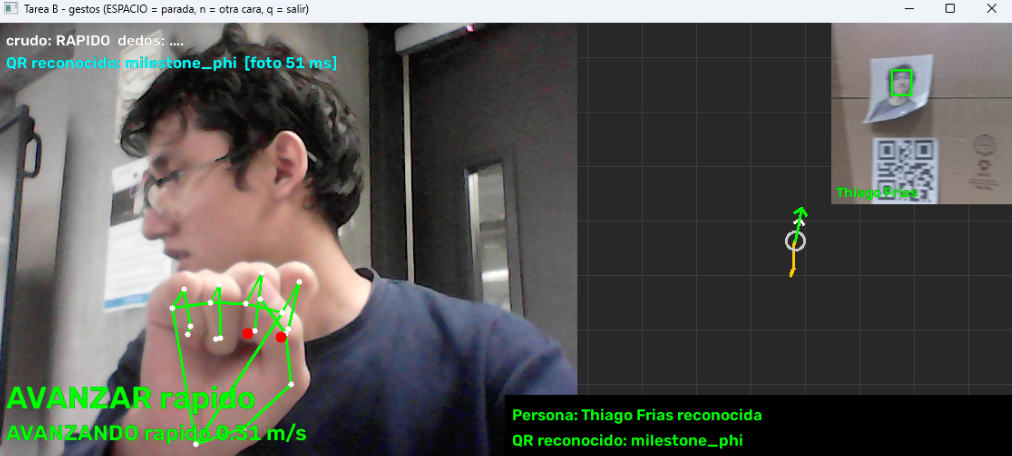
\includegraphics[width=\linewidth]{avanzar_rapido.png}
    \caption{Puño, avanza rápido.}
  \end{subfigure}
  \hfill
  \begin{subfigure}[t]{0.32\linewidth}
    \centering
    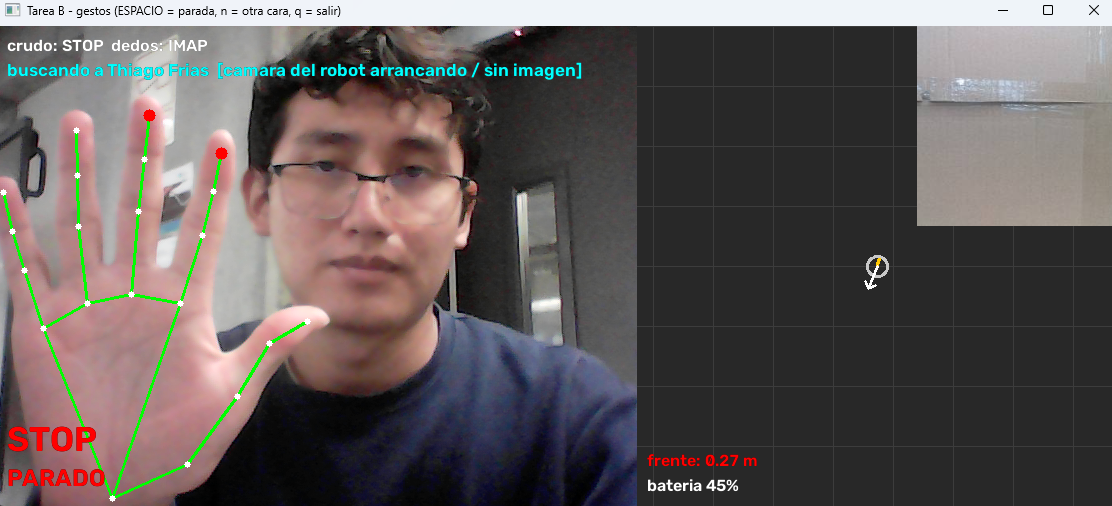
\includegraphics[width=\linewidth]{stop.png}
    \caption{Mano abierta, STOP.}
  \end{subfigure}
  \caption{Ventana de la Tarea~B con cada gesto. Se ven la mano detectada, la acción vigente del robot, la odometría y la distancia libre al frente.}
  \label{fig:gestos}
\end{figure}

\subsubsection{Estrategia de teleoperación}

El gesto confirmado se traduce en velocidades $(v, \omega)$ mediante una máquina de estados con tres estados, parado, girando y avanzando. El robot arranca parado y solo se mueve tras una orden explícita. Las órdenes de giro son relativas a hacia dónde mira el robot, como si la persona fuera el robot. Con cada señal se calcula un rumbo objetivo que se suma al rumbo anterior y no a la orientación actual, de modo que dos giros de $90^\circ$ seguidos suman exactamente $180^\circ$ sin acumular el error del primero. Tras una parada, el rumbo se cuenta desde la orientación en que quedó el robot.

El giro se hace en lazo cerrado con la odometría, con un control proporcional sobre el error de rumbo $e = \theta_{\mathrm{obj}} - \theta$,
\begin{equation}
  \omega = \operatorname{sat}\!\left(k_g\, e\right), \qquad v = 0,
\end{equation}
donde $\operatorname{sat}$ limita la velocidad angular a \SI{0,6}{\radian\per\second}, con un mínimo de \SI{0,15}{\radian\per\second} para vencer la fricción. El giro termina cuando $\lvert e\rvert \le 3^\circ$ y el robot queda quieto, y para avanzar la persona debe hacer una V o un puño. Mientras avanza, una corrección proporcional del mismo error, limitada a \SI{0,5}{\radian\per\second}, mantiene el rumbo.

La parada tiene prioridad sobre cualquier otro gesto y actúa incluso a mitad de un giro. Señalar mientras el robot avanza lo detiene y lo hace girar, y hacer una V o un puño mientras gira termina primero el giro y después avanza. Mantener una señal no repite el giro, y para girar de nuevo hay que bajar la mano y volver a señalar. Como sin mano el robot sigue con la última orden, la persona debe hacer una parada antes de bajar la mano. La barra espaciadora funciona como parada de emergencia, el robot se detiene si la cámara deja de entregar imágenes, y conserva el freno por LiDAR ante obstáculos frontales. Toda la teleoperación se hace solo con visión, sin teclado, ratón ni mando, como exige el enunciado.

\subsubsection{Anuncio del resultado}

En la Tarea~B el reconocimiento de la persona y del QR no mueve al robot, porque el desplazamiento es manual, incluido el regreso a A. Un hilo pide fotos a la cámara del robot de forma continua, unas cuatro por segundo, y otro las procesa, siempre con la más reciente. En cada foto detectamos el rostro e identificamos a la persona con la votación descrita antes. Una vez identificada, el sistema busca sin límite de tiempo el QR ubicado debajo de su rostro. El resultado se anuncia en dos pasos, primero el nombre y después el texto del QR. Como el TurtleBot~4 Lite no tiene altavoz, el anuncio se dice por voz en la computadora y se muestra en un cartel en pantalla. Si se indica a la persona por nombre, las demás caras se descartan.

\subsection{Decisiones de diseño y \textit{trade-offs}}

La Tabla~\ref{tab:tradeoffs} resume las decisiones principales. Tomamos la opción rápida cuando otra capa del sistema acotaba su riesgo y la conservadora cuando un error se penaliza directamente.

\begin{table}[!htbp]
  \centering
  \caption{Decisiones de diseño principales.}
  \label{tab:tradeoffs}
  \tabestilo
  \rowcolors{2}{cZebra}{white}
  \begin{tabular}{L{3.0cm}L{5.4cm}L{6.1cm}}
    \toprule
    \rowcolor{cAcc}\cab{Aspecto} & \cab{Decisión} & \cab{Compromiso} \\
    Procesamiento & Tarea A en la Raspberry y Tarea B en la PC & La Raspberry no depende del Wi-Fi, y procesa solo unas 2 fotos por segundo \\
    Mapa & Odometría y relocalización por ICP & Más robusto que BreezySLAM a alta velocidad, y la deriva no se corrige en la ida \\
    Búsqueda & Bandera y vuelta lenta en la meta, con fila y fronteras de respaldo & Ve las fotos sin recorrerlas todas, y depende de detectar la bandera \\
    Velocidad & Ida a \SI{0,30}{\meter\per\second} y vuelta turbo a \SI{0,45}{\meter\per\second} & Vuelta \SI{28}{\percent} más rápida en simulación, sin el límite de la Create~3 \\
    Detección de caras & Imagen ampliada a 500 píxeles & Cuatro veces más cálculo, y ve caras de 12 píxeles \\
    Reflejo en ArcFace & Solo en la Tarea~B & La mitad de cálculo en la A por menos de un punto de acierto \\
    Confirmación & Ranking y confirmación de cerca con foto HD & Unos \SI{4}{\second} por foto HD, y no se decide con caras de 14 a 25 píxeles \\
    Nombre y palabra & Votación de frente y lecturas repetidas & Más tiempo en la meta, y sin respuestas dudosas \\
    Gestos & Reglas geométricas sobre MediaPipe & Sin entrenamiento, y limitado a gestos por dedos estirados \\
    \bottomrule
  \end{tabular}
\end{table}

La decisión más importante fue no usar la exploración por fronteras como estrategia principal. Es ordenada y lenta, y con una cámara de $42^\circ$ un mapa completo no garantiza haber mirado la pared de la foto. La bandera nos dice dónde está la meta sin explorar, y la vuelta lenta frente a ella muestra casi todas las fotos. Para probar sin el robot, que se compartía entre grupos, construimos un simulador con LiDAR, odometría con ruido, el freno del puente y una cámara en perspectiva con fotos reales de la galería.

% =====================================================================
\section{Experimentos y resultados}
% =====================================================================

\subsection{Protocolo experimental}

Validamos el sistema en tres niveles. Empezamos por un simulador propio con LiDAR y odometría con ruido, el freno del puente y una cámara en perspectiva que dibuja fotos reales de la galería, excluidas al reconocer. Después pasamos al robot real, en sesiones del laboratorio los días 17, 19 y 21 de noviembre, y por último probamos el reconocimiento facial y los gestos sin el robot.

El simulador usa los tiempos de la Raspberry (una foto de vista previa cada unos \SI{0,5}{\second} con \SI{0,45}{\second} de retraso, y una foto HD cada unos \SI{4}{\second}), cajas de cartón con texturas y desenfoque al girar. El banco de pruebas corre la carrera completa en circuitos \texttt{tubo:N}. Cada circuito tiene de uno a tres giros con una señal en cada uno, cajas en los pasillos y, al final, un tubo con la bandera al fondo y cuatro fotos con su QR, junto con distractores como discos rojos, lisos y señales de prohibido. Cada semilla $N$ da un circuito que el programa no conoce. Probamos 32 circuitos en condiciones normales y 16 en condiciones difíciles, con odometría con error sistemático de hasta $\pm\SI{4}{\percent}$, más ruido y una cámara más lenta. En todos usamos el modo turbo y el límite de 3 minutos. Una carrera es exitosa si vuelve a menos de \SI{35}{\centi\meter} de A y anuncia la palabra correcta.

Para el reconocimiento dejamos una foto fuera de la galería y la «fotografiamos» como la vería el robot, con la cara de $N$ píxeles, menos contraste, desenfoque, ruido y JPEG, en 1320 cuadros por tamaño. Los gestos se verificaron con pruebas unitarias y en vivo con el robot.

\subsection{Métricas de evaluación}

El puntaje de cada tarea completada es
\begin{equation}
  P_{\mathrm{tarea}} = 4{,}5\cdot\frac{t_{\max} - t}{t_{\max} - t_{\min}},
\end{equation}
donde $t$ es el tiempo del equipo con penalizaciones, y $t_{\min}$ y $t_{\max}$ son el mejor y el peor tiempo entre los equipos que completaron la tarea. El puntaje total es $P = P_{\text{Tarea A}} + P_{\text{Tarea B}}$. Como el puntaje depende de los demás equipos, medimos la tasa de éxito, el tiempo total, el tiempo en reconocer a la persona, los choques y los nombres o palabras equivocados, que se penalizan. La competencia aún no se realiza, así que los tiempos del equipo se presentan en la exposición.

\subsection{Resultados de la Tarea A}

La Tabla~\ref{tab:sim} resume el banco, donde en condiciones normales las 32 carreras fueron exitosas, sin choques ni respuestas equivocadas. La mediana fue de \SI{87,9}{\second}, con un mínimo de \SI{48,9}{\second} y un máximo de \SI{153,2}{\second}, dentro del límite. La bandera se confirmó a los \SI{20}{\second}, la vuelta de la meta terminó a los \SI{49}{\second} (en las 27 carreras que la completaron) y la persona se reconoció a los \SI{62}{\second}. La vuelta vio en mediana 2,5 de las 4 fotos. En 9 carreras hizo falta el respaldo FILA, 29 confirmaron con foto HD y 7 llegaron a la foto buscada por descarte. El QR se leyó bien en las 32, y en 29 bastó una lectura.

\begin{table}[!htbp]
  \centering
  \caption{Resultados del banco de pruebas de la Tarea~A en el simulador, con los tiempos de la Raspberry y el modo turbo.}
  \label{tab:sim}
  \tabestilo\setlength{\tabcolsep}{3.5pt}
  \rowcolors{2}{cZebra}{white}
  \begin{tabular}{L{2.8cm}C{2.2cm}C{3.0cm}C{2.2cm}C{1.6cm}C{2.3cm}}
    \toprule
    \rowcolor{cAcc}\cab{Condiciones} & \cab{Éxitos} & \cab{Tiempo total (s), mediana (mín. a máx.)} & \cab{Reconocida a los (s), mediana} & \cab{Choques} & \cab{Equivocados} \\
    Normales, 32 circuitos & 32/32 (\SI{100}{\percent}) & \num{87,9} (\num{48,9} a \num{153,2}) & \num{61,9} & 0 & 0 \\
    Difíciles, 16 circuitos & 13/16 (\SI{81}{\percent}) & \num{121,5} (\num{53,5} a \num{165,5}) & \num{102,0} & 0 & 0 \\
    \bottomrule
  \end{tabular}
\end{table}

En condiciones difíciles fallaron tres carreras, y en las tres el nombre y la palabra eran correctos. Dos terminaron a más de \SI{35}{\centi\meter} de A porque la odometría las engañó, aunque según ella estaban a unos \SI{0,2}{\meter}. La tercera no encontró paso en la vuelta y agotó los 3 minutos. El riesgo principal es entonces la deriva de la odometría al regresar, que la relocalización por ICP corrige solo en parte. La Figura~\ref{fig:circuito} muestra una carrera completa en un circuito de $3{,}3\times3{,}3$~m.

\begin{figure}[!htbp]
  \centering
  \begin{tikzpicture}[x=17mm, y=17mm]
    % generado por scripts/figuras.py: mundo tubo:3 y la ruta verdadera de figuras/datos/tubo_traza.json
\draw[pared] (1.95,-2.8) -- (2.85,-2.8);
\draw[pared] (-0.45,-0.45) -- (1.95,-0.45);
\draw[pared] (0.95,0.1) -- (1.3,0.1);
\draw[pared] (1.65,0.15) -- (1.9,0.15);
\draw[pared] (-0.45,0.45) -- (0.95,0.45);
\draw[pared] (1.3,0.45) -- (1.65,0.45);
\draw[pared] (1.9,0.45) -- (2.85,0.45);
\draw[pared] (-0.45,-0.45) -- (-0.45,0.45);
\draw[pared] (0.95,0.1) -- (0.95,0.45);
\draw[pared] (1.3,0.1) -- (1.3,0.45);
\draw[pared] (1.65,0.15) -- (1.65,0.45);
\draw[pared] (1.9,0.15) -- (1.9,0.45);
\draw[pared] (1.95,-2.8) -- (1.95,-0.45);
\draw[pared] (2.85,-2.8) -- (2.85,0.45);
\draw[pared] (0.939,0.103) -- (1.286,0.103);
\draw[pared] (1.286,0.103) -- (1.286,0.45);
\draw[pared] (1.286,0.45) -- (0.939,0.45);
\draw[pared] (0.939,0.45) -- (0.939,0.103);
\draw[pared] (1.627,0.155) -- (1.922,0.155);
\draw[pared] (1.922,0.155) -- (1.922,0.45);
\draw[pared] (1.922,0.45) -- (1.627,0.45);
\draw[pared] (1.627,0.45) -- (1.627,0.155);
\node[senal] (senal) at (2.846,-0.054) {};
\node[bandera] (bandera) at (2.366,-2.796) {};
\node[buscada] at (2.85,-0.991) {};
\node[foto] at (1.95,-1.01) {};
\node[foto] at (1.95,-1.54) {};
\node[foto] at (2.85,-2.028) {};
\draw[tIda] (-0.098,-0) -- (-0.033,-0.002) -- (0.057,-0.005) -- (0.147,-0.007) -- (0.237,-0.011) -- (0.327,-0.019) -- (0.416,-0.033) -- (0.504,-0.049) -- (0.593,-0.065) -- (0.682,-0.081) -- (0.77,-0.097) -- (0.859,-0.113) -- (0.947,-0.129) -- (1.036,-0.144) -- (1.125,-0.153) -- (1.215,-0.157) -- (1.305,-0.159) -- (1.395,-0.161) -- (1.485,-0.163) -- (1.575,-0.164) -- (1.665,-0.166) -- (1.755,-0.168) -- (1.845,-0.17) -- (1.935,-0.172) -- (2.025,-0.173) -- (2.115,-0.175) -- (2.203,-0.177) -- (2.289,-0.168) -- (2.35,-0.151) -- (2.401,-0.146) -- (2.433,-0.158) -- (2.452,-0.178) -- (2.472,-0.216) -- (2.496,-0.288) -- (2.513,-0.377) -- (2.523,-0.466) -- (2.53,-0.556) -- (2.536,-0.646) -- (2.543,-0.736) -- (2.545,-0.765);
\draw[tFila] (2.545,-0.765) -- (2.547,-0.84) -- (2.546,-0.915) -- (2.542,-0.99) -- (2.538,-1.065) -- (2.534,-1.14) -- (2.531,-1.215) -- (2.527,-1.29) -- (2.523,-1.365) -- (2.52,-1.44) -- (2.516,-1.515) -- (2.512,-1.589) -- (2.507,-1.664) -- (2.501,-1.739) -- (2.494,-1.814) -- (2.483,-1.888) -- (2.468,-1.961) -- (2.456,-2.01) -- (2.456,-2.01) -- (2.456,-2.01) -- (2.456,-2.01) -- (2.456,-2.01) -- (2.456,-2.01) -- (2.456,-2.01) -- (2.456,-2.01) -- (2.456,-2.01) -- (2.456,-2.01) -- (2.456,-2.01) -- (2.456,-2.01) -- (2.456,-2.01) -- (2.456,-2.01) -- (2.456,-2.01) -- (2.456,-2.01) -- (2.456,-2.01) -- (2.456,-2.01) -- (2.456,-2.01) -- (2.456,-2.01) -- (2.456,-2.01) -- (2.456,-2.01) -- (2.456,-2.01) -- (2.456,-2.01) -- (2.456,-2.01) -- (2.456,-2.01) -- (2.456,-2.01) -- (2.456,-2.01) -- (2.456,-2.01) -- (2.456,-2.01) -- (2.456,-2.01) -- (2.456,-2.01) -- (2.456,-2.01) -- (2.456,-2.01) -- (2.456,-2.01) -- (2.456,-2.01) -- (2.456,-2.01) -- (2.456,-2.01) -- (2.456,-2.01) -- (2.456,-2.01) -- (2.456,-2.01) -- (2.456,-2.01) -- (2.456,-2.01) -- (2.456,-2.01) -- (2.456,-2.01) -- (2.456,-2.01) -- (2.456,-2.01) -- (2.456,-2.01) -- (2.456,-2.01) -- (2.456,-2.01) -- (2.456,-2.01) -- (2.456,-2.01) -- (2.456,-2.01) -- (2.456,-2.01) -- (2.456,-2.01) -- (2.456,-2.01) -- (2.456,-2.01) -- (2.456,-2.01) -- (2.456,-2.01) -- (2.456,-2.01) -- (2.456,-2.01) -- (2.456,-2.01) -- (2.456,-2.01) -- (2.456,-2.01) -- (2.456,-2.01) -- (2.456,-2.01) -- (2.456,-2.01) -- (2.456,-2.01) -- (2.456,-2.01) -- (2.456,-2.01) -- (2.456,-2.01) -- (2.456,-2.01) -- (2.456,-2.01) -- (2.456,-2.01) -- (2.456,-2.01) -- (2.456,-2.01) -- (2.456,-2.01) -- (2.456,-2.01) -- (2.442,-2.02) -- (2.414,-2.03) -- (2.389,-2.026) -- (2.372,-2.014) -- (2.36,-2) -- (2.352,-1.984) -- (2.349,-1.978);
\draw[tQr] (2.349,-1.978) -- (2.349,-1.978) -- (2.349,-1.978) -- (2.349,-1.978) -- (2.349,-1.978) -- (2.349,-1.978) -- (2.349,-1.978) -- (2.349,-1.978) -- (2.349,-1.978) -- (2.349,-1.978) -- (2.349,-1.978) -- (2.349,-1.978) -- (2.349,-1.978) -- (2.349,-1.978) -- (2.349,-1.978);
\draw[tFila] (2.349,-1.978) -- (2.37,-2.002) -- (2.394,-2.029) -- (2.417,-2.056) -- (2.436,-2.078) -- (2.414,-2.038) -- (2.388,-1.968) -- (2.373,-1.895) -- (2.363,-1.82) -- (2.359,-1.746) -- (2.356,-1.671) -- (2.354,-1.596) -- (2.352,-1.521) -- (2.352,-1.471) -- (2.355,-1.464) -- (2.384,-1.438) -- (2.421,-1.43) -- (2.449,-1.438) -- (2.465,-1.455) -- (2.484,-1.497) -- (2.501,-1.568) -- (2.501,-1.583) -- (2.501,-1.583) -- (2.501,-1.583) -- (2.501,-1.583) -- (2.501,-1.583) -- (2.501,-1.583) -- (2.501,-1.583) -- (2.501,-1.583) -- (2.494,-1.584) -- (2.441,-1.6) -- (2.404,-1.63) -- (2.373,-1.677) -- (2.344,-1.745) -- (2.325,-1.817) -- (2.313,-1.891) -- (2.306,-1.966) -- (2.302,-2.041) -- (2.299,-2.116) -- (2.296,-2.191) -- (2.295,-2.253) -- (2.296,-2.278) -- (2.296,-2.278) -- (2.296,-2.278) -- (2.296,-2.278) -- (2.296,-2.278) -- (2.296,-2.278) -- (2.296,-2.278) -- (2.296,-2.278) -- (2.299,-2.278) -- (2.354,-2.276) -- (2.396,-2.257) -- (2.424,-2.227) -- (2.447,-2.186) -- (2.448,-2.184) -- (2.448,-2.184) -- (2.448,-2.184) -- (2.448,-2.184) -- (2.448,-2.184) -- (2.448,-2.184) -- (2.448,-2.184) -- (2.448,-2.184) -- (2.448,-2.184) -- (2.417,-2.178) -- (2.385,-2.16) -- (2.36,-2.131) -- (2.335,-2.082) -- (2.313,-2.01) -- (2.3,-1.937) -- (2.291,-1.862) -- (2.287,-1.787) -- (2.288,-1.737) -- (2.288,-1.737) -- (2.288,-1.737) -- (2.288,-1.737) -- (2.288,-1.737) -- (2.288,-1.737) -- (2.288,-1.737) -- (2.288,-1.737) -- (2.288,-1.737) -- (2.323,-1.73) -- (2.371,-1.705) -- (2.406,-1.663) -- (2.437,-1.596) -- (2.456,-1.524) -- (2.466,-1.45) -- (2.468,-1.409) -- (2.469,-1.391) -- (2.469,-1.39);
\draw[tQr] (2.469,-1.39) -- (2.469,-1.39) -- (2.469,-1.39) -- (2.469,-1.39) -- (2.469,-1.39) -- (2.469,-1.39) -- (2.469,-1.39) -- (2.469,-1.39) -- (2.469,-1.39) -- (2.469,-1.39) -- (2.469,-1.39) -- (2.469,-1.39) -- (2.469,-1.39) -- (2.469,-1.39) -- (2.469,-1.39) -- (2.469,-1.39) -- (2.469,-1.39) -- (2.469,-1.39);
\draw[tFila] (2.469,-1.39) -- (2.447,-1.413) -- (2.422,-1.439) -- (2.397,-1.465) -- (2.372,-1.49) -- (2.381,-1.477) -- (2.413,-1.41) -- (2.434,-1.338) -- (2.448,-1.265) -- (2.455,-1.215);
\draw[tVuelta] (2.455,-1.215) -- (2.464,-1.105) -- (2.47,-0.971) -- (2.477,-0.836) -- (2.483,-0.701) -- (2.468,-0.567) -- (2.421,-0.441) -- (2.346,-0.329) -- (2.266,-0.254) -- (2.216,-0.224) -- (2.162,-0.203) -- (2.071,-0.18) -- (1.939,-0.153) -- (1.812,-0.136) -- (1.742,-0.131) -- (1.623,-0.129) -- (1.488,-0.129) -- (1.353,-0.129) -- (1.218,-0.129) -- (1.083,-0.127) -- (0.948,-0.122) -- (0.813,-0.117) -- (0.678,-0.111) -- (0.544,-0.106) -- (0.409,-0.1) -- (0.303,-0.092) -- (0.214,-0.079) -- (0.142,-0.067) -- (0.096,-0.058) -- (0.096,-0.058) -- (0.096,-0.058) -- (0.096,-0.058) -- (0.096,-0.058);
\node[puntoA] (A) at (-0.1,0) {};
% caja: x -0.45..2.85  y -2.80..0.45

    \node[font=\small\bfseries, text=cInk, left=0.8mm of A] {A};
    \node[font=\small\bfseries, text=cInk, anchor=north] at (2.37,-2.95) {B};
    \begin{scope}[shift={(3.35,-0.35)}, every node/.style={font=\footnotesize, anchor=west, text=cInk}]
      \draw[tIda] (0,0) -- (0.4,0);           \node at (0.5,0) {ida};
      \draw[tFila] (0,-0.38) -- (0.4,-0.38);   \node at (0.5,-0.38) {búsqueda en la meta};
      \draw[tQr] (0,-0.76) -- (0.4,-0.76);     \node at (0.5,-0.76) {reconocer y leer el QR};
      \draw[tVuelta] (0,-1.14) -- (0.4,-1.14); \node at (0.5,-1.14) {vuelta};
      \node[buscada] at (0.2,-1.52) {};        \node at (0.5,-1.52) {la persona buscada};
      \node[foto] at (0.2,-1.9) {};            \node at (0.5,-1.9) {otras fotos};
      \node[bandera] at (0.2,-2.28) {};        \node at (0.5,-2.28) {bandera (la meta)};
      \node[senal] at (0.2,-2.66) {};          \node at (0.5,-2.66) {señal de giro};
    \end{scope}
  \end{tikzpicture}
  \caption{Carrera simulada en un circuito en L, con el recorrido verdadero del robot por fases. Terminó en \SI{87,8}{\second}, sin choques.}
  \label{fig:circuito}
\end{figure}

En el robot real, la primera carrera dentro de la Raspberry (19 de noviembre), todavía con la búsqueda por fila, vio la señal a \SI{1,7}{\second}, giró a la derecha a los \SI{4,5}{\second}, reconoció a la persona correcta ($p = 0{,}96$), leyó su QR a los \SI{76}{\second} y paró a \SI{0,21}{\meter} de A a los \SI{93,9}{\second}, sin choques (Figura~\ref{fig:fases}). Entre 15 y \SI{50}{\second} recorrió la fila, porque la Raspberry procesa unas 2 fotos por segundo, y entre 52 y \SI{82}{\second} esperó frente al QR, porque cada foto HD tarda unos \SI{4}{\second}. Eso motivó la bandera y el uso de la HD solo cuando hace falta. El 21 de noviembre probamos la meta con bandera en el robot. La vuelta vio las cuatro fotos, aunque en la vista previa las caras medían solo 14 a 25 píxeles y no se distinguía a nadie, lo que llevó a confirmar de cerca con fotos HD (Sección~\ref{sec:fallos}). La meta con bandera completa solo se validó en simulación.

\begin{figure}[!htbp]
  \centering
  \begin{tikzpicture}[x=1mm, y=1mm]
    \fase{0}{15}{cIda}{ida}
    \fase{15}{52}{cFila}{buscar en la fila}
    \fase{52}{82}{cQr}{QR}
    \fase{82}{93.9}{cVuelta}{}
    \node[font=\small\bfseries, text=cInk, anchor=west] at ({93.9*0.9+2},3) {\SI{93,9}{\second}};
    \draw[cInk!40, line width=0.3pt] (0,-1.5) -- (85,-1.5);
    \foreach \t in {0,30,60,90}{\draw[cInk!40] ({\t*0.9},-1.5) -- ++(0,-1); \node[font=\scriptsize, text=cSrc, anchor=north] at ({\t*0.9},-2.5) {\t\,s};}
  \end{tikzpicture}
  \caption{Fases de la primera carrera con el robot real (19 de noviembre), todavía con la búsqueda por fila.}
  \label{fig:fases}
\end{figure}

\subsection{Resultados de la Tarea B}

La Tarea~B depende de quién conduce y del circuito, así que no medimos un tiempo antes de la competencia. Verificamos que cada gesto produce la acción esperada de dos formas. La primera son 24 pruebas unitarias del clasificador, del estabilizador y de la máquina de estados, que cubren por ejemplo que STOP frena en pleno giro en 2 cuadros y que mantener una señal no repite el giro. La segunda es en vivo, con el robot real y la webcam. La Figura~\ref{fig:gestos} reúne capturas de esas pruebas, con el gesto detectado, la acción vigente, la odometría, la distancia libre al frente y la batería.

\subsection{Resultados del reconocimiento facial y del QR}
\label{sec:res_cara}

La Tabla~\ref{tab:acierto} y la Figura~\ref{fig:acierto} muestran el acierto según el tamaño de la cara. Con 24 píxeles o más el acierto por foto es de al menos \SI{95,8}{\percent}, y votando con varias fotos llega a \SI{99,1}{\percent}. Con 14 a 18 píxeles baja a \num{73} a \SI{86}{\percent} por foto, y la votación lo sube solo a \num{83} a \SI{91}{\percent}. Por eso el robot no decide con caras tan chicas, se acerca hasta que la cara mide al menos 24 píxeles y, si en la vista previa mide menos de 40, la confirma con una foto HD. El reflejo cambia el acierto en menos de 1,5 puntos y duplica el costo de ArcFace.

\begin{table}[!htbp]
  \centering
  \caption{Acierto del reconocimiento (MobileFaceNet, galería de 20 personas, 1320 cuadros por tamaño). «Voto» es el acierto votando con las 4 fotos de cada prueba.}
  \label{tab:acierto}
  \tabestilo
  \rowcolors{3}{cZebra}{white}
  \begin{tabular}{cccccc}
    \toprule
    \rowcolor{cAcc} & & \multicolumn{2}{c}{\cab{Con reflejo (Tarea B)}} & \multicolumn{2}{c}{\cab{Sin reflejo (Tarea A)}} \\
    \arrayrulecolor{white}\cmidrule(lr){3-4}\cmidrule(lr){5-6}\arrayrulecolor{cAcc}
    \rowcolor{cAcc}\cab{Cara (px)} & \cab{Detecta} & \cab{1 foto} & \cab{Voto} & \cab{1 foto} & \cab{Voto} \\
    14 & \SI{98,1}{\percent} & \SI{74,5}{\percent} & \SI{83,2}{\percent} & \SI{73,1}{\percent} & \SI{82,6}{\percent} \\
    18 & \SI{99,5}{\percent} & \SI{86,5}{\percent} & \SI{90,0}{\percent} & \SI{85,4}{\percent} & \SI{90,6}{\percent} \\
    24 & \SI{100}{\percent} & \SI{96,2}{\percent} & \SI{99,1}{\percent} & \SI{95,8}{\percent} & \SI{99,1}{\percent} \\
    32 & \SI{100}{\percent} & \SI{98,9}{\percent} & \SI{99,7}{\percent} & \SI{99,0}{\percent} & \SI{99,7}{\percent} \\
    48 & \SI{100}{\percent} & \SI{99,2}{\percent} & \SI{100}{\percent} & \SI{99,2}{\percent} & \SI{100}{\percent} \\
    \bottomrule
  \end{tabular}
\end{table}

\begin{figure}[!htbp]
  \centering
  \begin{tikzpicture}
    \begin{axis}[sobrio, width=0.6\linewidth, height=5.2cm, xmin=12, xmax=50, ymin=70, ymax=101,
        xlabel={tamaño de la cara (px)}, ylabel={acierto (\%)}, xtick={14,18,24,32,48}, ytick={70,80,90,100},
        grid=major, legend pos=south east, legend cell align=left, mark size=1.6pt]
      \addplot[cMuted, mark=*] coordinates {(14,73.1) (18,85.4) (24,95.8) (32,99.0) (48,99.2)};
      \addlegendentry{1 foto}
      \addplot[cAcc, mark=*] coordinates {(14,82.6) (18,90.6) (24,99.1) (32,99.7) (48,100)};
      \addlegendentry{votando 4 fotos}
      \addplot[cCelD, dashed, no marks, line width=0.7pt] coordinates {(24,70) (24,101)};
      \addlegendentry{24 px: mínimo para decidir}
      \addplot[cCelD, densely dotted, no marks, line width=0.9pt] coordinates {(40,70) (40,101)};
      \addlegendentry{40 px: sin foto HD}
    \end{axis}
  \end{tikzpicture}
  \caption{Acierto según el tamaño de la cara, sin reflejo (Tarea~A). Las líneas punteadas son los umbrales del robot, 24 píxeles para decidir y 40 para no pedir foto HD.}
  \label{fig:acierto}
\end{figure}

En el simulador el QR se leyó bien en las 32 carreras normales y en las 16 difíciles, sin palabras equivocadas. En el robot real, el 19 de noviembre el QR se leyó una vez y la regla de entonces pedía dos, así que se anunció solo el nombre. Desde entonces basta una lectura si la cara mide al menos 35 píxeles.

\subsection{Análisis de fallos y casos límite}
\label{sec:fallos}

La Tabla~\ref{tab:fallos} resume lo que falló con el robot real y cómo lo corregimos. Casi todos los fallos aparecieron solo en el hardware, y varios no tenían relación con la visión, como un bloqueo entre hilos, un conflicto de versiones de una librería y un paquete UDP perdido. Entre los casos límite, el robot falla en pasos de unos \SI{0,48}{\meter} con un giro cerrado, porque el freno del puente se activa a \SI{0,28}{\meter} y en un cruce tan estrecho todo queda bajo esa distancia.

\begin{table}[!htbp]
  \centering
  \caption{Fallos encontrados con el robot real y su corrección.}
  \label{tab:fallos}
  \tabestilo
  \rowcolors{2}{cZebra}{white}
  \begin{tabular}{L{1.0cm}L{4.3cm}L{4.5cm}L{4.5cm}}
    \toprule
    \rowcolor{cAcc}\cab{Fecha} & \cab{Síntoma} & \cab{Causa} & \cab{Corrección} \\
    19/11 & El puente no responde tras la partida & Un hilo bloqueaba a otro con un \textit{lock} & \textit{Lock} reentrante \\
    19/11 & La carrera corre sin cámara & Una versión nueva de \texttt{numpy} rompía el puente & El puente corre sin los paquetes del usuario \\
    19/11 & La palabra no llega a la computadora & Se enviaba en un solo paquete UDP & Se repite durante \SI{3}{\second} \\
    19/11 & Anuncia solo el nombre & El QR se leyó 1 vez y se pedían 2 & Basta una lectura con una cara de 35 píxeles o más \\
    21/11 & Ve las 4 fotos y no reconoce a nadie & Las caras miden 14 a 25 píxeles en la vista previa & Confirmar de cerca con foto HD si mide menos de 40 píxeles \\
    21/11 & El puente deja de responder & Un error del \textit{logger} mataba el hilo UDP & El registro ya no puede tumbar el hilo \\
    21/11 & Dice un nombre con $p = 0{,}10$ & El ranking aceptaba una foto con $p$ baja & De cerca exige $p \ge 0{,}45$, y si no queda dudosa \\
    21/11 & Va a caras del laboratorio y a banderas falsas & Cualquier cara contaba & Solo caras cerca de la bandera y a menos de \SI{0,5}{\meter} del piso \\
    21/11 & Una señal girada $180^\circ$ se lee al revés & Girada se parece a una «J», que se leía como izquierda & Se corrigió el detector y se agregó una prueba \\
    \bottomrule
  \end{tabular}
\end{table}

% =====================================================================
\section{Discusión}
% =====================================================================

\subsection{Interpretación de los resultados}

Los resultados muestran dos cosas. La primera es que la estrategia generaliza a circuitos desconocidos, ya que las 32 carreras normales terminaron bien, sin choques ni respuestas equivocadas, y las 16 difíciles bajaron a \SI{81}{\percent}. En las tres fallas el nombre y la palabra fueron correctos, lo que indica que el reconocimiento es robusto y que el punto débil es el regreso con la odometría deteriorada. La segunda es que el reconocimiento depende mucho del tamaño de la cara. Por encima de 24 píxeles es casi perfecto, y por debajo cae con rapidez. De esa curva salen los umbrales del robot (24 píxeles para decidir y 40 para no pedir HD), y lo del 21 de noviembre mostró que ignorarlos lleva a no reconocer a nadie.

El tiempo se reparte distinto a lo esperado. En la primera carrera real, la fila de fotos y el QR ocupaban casi todo el tiempo. La mediana simulada de \SI{88}{\second} es del mismo orden que los \SI{94}{\second} de aquella carrera, aunque no son comparables, ya que una es simulación y la otra un solo intento real con otra meta. La mayor ganancia viene de no recorrer todas las fotos. Cuando se introdujo la bandera, en los mismos 16 circuitos los éxitos subieron de 8 a 15 y la mediana bajó de \SI{135}{\second} a \SI{82}{\second}. El turbo acorta además la vuelta un \SI{28}{\percent}. En la Tarea~B, las reglas geométricas distinguen bien la mano abierta, el puño y la V sin entrenar ningún modelo, y el filtrado temporal evita que un cuadro con ruido mueva el robot.

\subsection{Limitaciones}

Gran parte de la validación se hizo en simulación, que es 2D y no modela el deslizamiento de las ruedas ni la iluminación, y el robot estuvo disponible en pocas sesiones. La meta con bandera y el turbo se ajustaron con pruebas parciales del 21 de noviembre y solo se validaron completos en simulación, donde se midió la ganancia del turbo. La cámara está a \SI{13}{\centi\meter} del suelo, así que las fotos altas se ven pequeñas, y su campo de visión no se midió con precisión. La Raspberry procesa unas 2 fotos por segundo y la foto HD tarda unos \SI{4}{\second}. El LiDAR 2D no ve obstáculos bajos ni vidrio, y el freno solo vigila el frente. La Tarea~A corrige la deriva solo al volver y falla en pasos de unos \SI{0,48}{\meter} con giro cerrado.

Por otro lado, el reconocimiento depende de una galería pequeña con fotos de un solo día y siempre responde con alguien de ella. El detector de la bandera se ajustó con fotos del laboratorio y supone que la hoja va sobre cartón. Si la meta del día no trae bandera, el robot usa los respaldos, que en un circuito antiguo de seis fotos sin bandera completaron la carrera en \SI{114}{\second} en simulación, con menos margen. En la Tarea~B, sin mano el robot sigue con la última orden.

\subsection{Lecciones aprendidas}

\begin{itemize}
  \item \textbf{Probar pronto en el robot.} Un bloqueo entre hilos, un conflicto de versiones de \texttt{numpy} y un anuncio UDP perdido solo aparecieron en el hardware real. El 21 de noviembre las caras medían 14 a 25 píxeles, mucho menos de lo que suponía el simulador.
  \item \textbf{Medir antes de optimizar.} El cuello de botella era la ventana dinámica en Python y no las redes, y optimizarla la hizo seis veces más rápida (de 12 a \SI{2}{\milli\second}).
  \item \textbf{Ajustar el simulador a la realidad.} Con los tiempos de la Raspberry y fotos como las del laboratorio aparecieron problemas ocultos, y las heurísticas ajustadas con ese simulador subieron el acierto del banco de 5 a 11 de 12 circuitos.
  \item \textbf{Preferir decisiones seguras.} Decidir el nombre con fotos chicas causó errores, y exigir alta probabilidad, vistas de frente y confirmación de cerca los eliminó.
  \item \textbf{Separar la seguridad de la decisión.} El freno en el robot permitió probar estrategias agresivas, como el turbo, sin riesgo.
\end{itemize}

\subsection{Trabajo futuro}

\begin{itemize}
  \item Validar el turbo y la vuelta de la meta con fotos HD (una opción experimental) en carreras completas con el robot real.
  \item Detectar caras en el procesador de la cámara OAK-D para liberar la Raspberry.
  \item Usar un SLAM con cierre de bucles para corregir la deriva también en la ida.
  \item Calibrar la cámara y ampliar la galería con fotos en otras condiciones.
  \item En la Tarea~B, detener el robot si no ve la mano durante un tiempo.
\end{itemize}

% =====================================================================
\section{Conclusiones}
% =====================================================================

Construimos un sistema para que un TurtleBot~4 vaya de A a B, reconozca a una persona entre varias fotografías, lea su QR y vuelva a A anunciando el resultado, de forma autónoma y por gestos. Ambas tareas comparten la comunicación UDP, el freno de emergencia y el módulo de reconocimiento.

En la Tarea~A, los carriles reactivos con una ventana dinámica permitieron priorizar el tiempo sin perder seguridad. La bandera de la meta, con una vuelta lenta y la confirmación de cerca con fotos HD, permitió ver las fotos sin recorrerlas, y el turbo y la relocalización por ICP aceleraron y corrigieron el regreso. En simulación, las 32 carreras normales terminaron bien, con una mediana de \SI{87,9}{\second} y sin choques ni respuestas equivocadas. En la Tarea~B, reglas geométricas sobre MediaPipe con filtrado temporal y una máquina de estados permitieron conducir solo con la mano. En el reconocimiento, YuNet y ArcFace con votación entre fotos dieron decisiones confiables con caras de 24 píxeles o más, y asignar cada QR a su cara permitió leer solo el de la persona buscada. La lección principal es que el sistema se valida en el robot, ya que el simulador aceleró el desarrollo y el hardware real obligó a ajustar muchas decisiones.


% =====================================================================
%  Bibliografía
% =====================================================================
\clearpage
\begin{thebibliography}{99}

\bibitem{thrun2005} S.~Thrun, W.~Burgard y D.~Fox, \textit{Probabilistic Robotics}. MIT Press, 2005.

\bibitem{steux2010} B.~Steux y O.~El~Hamzaoui, ``tinySLAM: A SLAM algorithm in less than 200 lines C-language program,'' en \textit{Proc. ICARCV}, 2010.

\bibitem{yamauchi1997} B.~Yamauchi, ``A frontier-based approach for autonomous exploration,'' en \textit{Proc. IEEE CIRA}, 1997.

\bibitem{dijkstra1959} E.~W. Dijkstra, ``A note on two problems in connexion with graphs,'' \textit{Numerische Mathematik}, vol.~1, pp.~269--271, 1959.

\bibitem{hart1968} P.~E. Hart, N.~J. Nilsson y B.~Raphael, ``A formal basis for the heuristic determination of minimum cost paths,'' \textit{IEEE Trans. Systems Science and Cybernetics}, vol.~4, n.º~2, pp.~100--107, 1968.

\bibitem{coulter1992} R.~C. Coulter, ``Implementation of the pure pursuit path tracking algorithm,'' Carnegie Mellon University, Tech. Rep. CMU-RI-TR-92-01, 1992.

\bibitem{wu2023yunet} W.~Wu et~al., ``YuNet: A tiny millisecond-level face detector,'' \textit{Machine Intelligence Research}, 2023.

\bibitem{deng2019arcface} J.~Deng, J.~Guo, J.~Yang, N.~Xue, I.~Kotsia y S.~Zafeiriou, ``ArcFace: Additive angular margin loss for deep face recognition,'' \textit{IEEE Trans. Pattern Analysis and Machine Intelligence}, 2022.

\bibitem{chen2018mobilefacenets} S.~Chen, Y.~Liu, X.~Gao y Z.~Han, ``MobileFaceNets: Efficient CNNs for accurate real-time face verification on mobile devices,'' en \textit{Proc. CCBR}, 2018.

\bibitem{zhang2020mediapipehands} F.~Zhang et~al., ``MediaPipe Hands: On-device real-time hand tracking,'' \textit{arXiv:2006.10214}, 2020.

\end{thebibliography}

\end{document}
